% /*
%  * ----------------------------------------------------------------------------
%  * "THE BEER-WARE LICENSE" (Revision 42):
%  * <michi.wieland@hotmail.com> wrote this file. As long as you retain this notice you
%  * can do whatever you want with this stuff. If we meet some day, and you think
%  * this stuff is worth it, you can buy me a beer in return. Michael Wieland
%  * ----------------------------------------------------------------------------
%  */

\documentclass[
a4paper,
oneside,
10pt,
fleqn,
headsepline,
toc=listofnumbered, 
bibliography=totocnumbered]{scrartcl}

% deutsche Trennmuster etc.
\usepackage[T1]{fontenc}
\usepackage[utf8]{inputenc}
\usepackage[english, ngerman]{babel} % \selectlanguage{english} if  needed
\usepackage{lmodern} % use modern latin fonts

% Custom commands
\newcommand{\AUTHOR}{Michael Wieland}
\newcommand{\INSTITUTE}{Hochschule für Technik Rapperswil}
\newcommand{\GITHUB}{https://github.com/michiwieland/hsr-zusammenfassungen}
\newcommand{\LICENSEURL}{https://en.wikipedia.org/wiki/Beerware}
\newcommand{\LICENSE}{
"THE BEER-WARE LICENSE" (Revision 42):
<michi.wieland@hotmail.com> wrote this file. As long as you retain this notice you
can do whatever you want with this stuff. If we meet some day, and you think
this stuff is worth it, you can buy me a beer in return. Michael Wieland	
}

% Jede Überschrift 1 auf neuer Seite
\let\stdsection\section
\renewcommand\section{\clearpage\stdsection}

% Multiple Authors
\usepackage{authblk}

% Include external pdf
\usepackage{pdfpages}

% Layout / Seitenränder
\usepackage{geometry}

% Inhaltsverzeichnis
\usepackage{makeidx} 
\makeindex

\usepackage{url}
\usepackage[pdfborder={0 0 0}]{hyperref}
\usepackage[all]{hypcap}
\usepackage{hyperxmp} % for license metadata

% Glossar und Abkürzungsverzeichnis
\usepackage[acronym,toc,nopostdot]{glossaries}
\glossarystyle{altlist}
\usepackage{xparse}
\DeclareDocumentCommand{\newdualentry}{ O{} O{} m m m m } {
	\newglossaryentry{gls-#3}{
		name={#4 : #5},
		text={#5\glsadd{#3}},
		description={#6},
		#1
	}
	\makeglossaries
	\newacronym[see={[Siehe:]{gls-#3}},#2]{#3}{#4}{#5\glsadd{gls-#3}}
}
\makeglossaries

% Mathematik
\usepackage{amsmath}
\usepackage{amssymb}
\usepackage{amsfonts}
\usepackage{enumitem}

% Images
\usepackage{graphicx}
\graphicspath{{images/}} % default paths

% Boxes
\usepackage{fancybox}

%Tables
\usepackage{tabu}
\usepackage{booktabs} % toprule, midrule, bottomrule
\usepackage{array} % for matrix tables

% Multi Columns
\usepackage{multicol}

% Header and footer
\usepackage{scrlayer-scrpage}
\setkomafont{pagehead}{\normalfont}
\setkomafont{pagefoot}{\normalfont}
\automark*{section}
\clearpairofpagestyles
\ihead{\headmark}
\ohead{\AUTHOR}
\cfoot{\pagemark}

% Pseudocode
\usepackage{algorithmic}
\usepackage[linesnumbered,ruled]{algorithm2e}

% Code Listings
\usepackage{listings}
\usepackage{color}
\usepackage{beramono}

\definecolor{bluekeywords}{rgb}{0,0,1}
\definecolor{greencomments}{rgb}{0,0.5,0}
\definecolor{redstrings}{rgb}{0.64,0.08,0.08}
\definecolor{xmlcomments}{rgb}{0.5,0.5,0.5}
\definecolor{types}{rgb}{0.17,0.57,0.68}

\lstdefinestyle{visual-studio-style}{
	language=[Sharp]C,
	columns=flexible,
	showstringspaces=false,
	basicstyle=\footnotesize\ttfamily, 
	commentstyle=\color{greencomments},
	morekeywords={partial, var, value, get, set},
	keywordstyle=\bfseries\color{bluekeywords},
	stringstyle=\color{redstrings},
	breaklines=true,
	breakatwhitespace=true,
	tabsize=4,
	numbers=left,
	numberstyle=\tiny\color{black},
	frame=lines,
	showspaces=false,
	showtabs=false,
	escapeinside={£}{£},
}

\definecolor{DarkPurple}{rgb}{0.4, 0.1, 0.4}
\definecolor{DarkCyan}{rgb}{0.0, 0.5, 0.4}
\definecolor{LightLime}{rgb}{0.3, 0.5, 0.4}
\definecolor{Blue}{rgb}{0.0, 0.0, 1.0}

\lstdefinestyle{cevelop-style}{
	language=C++,  
	columns=flexible,
	showstringspaces=false,     
	basicstyle=\footnotesize\ttfamily, 
	keywordstyle=\bfseries\color{DarkPurple},
	commentstyle=\color{LightLime},
	stringstyle=\color{Blue}, 
	escapeinside={£}{£}, % latex scope within code      
	breaklines=true,
	breakatwhitespace=true,
	showspaces=false,
	showtabs=false,
	tabsize=4,
	morekeywords={include,ifndef,define},
	numbers=left,
	numberstyle=\tiny\color{black},
	frame=lines,
}

\lstdefinestyle{eclipse-style}{
	language=Java,  
	columns=flexible,
	showstringspaces=false,     
	basicstyle=\footnotesize\ttfamily, 
	keywordstyle=\bfseries\color{DarkPurple},
	commentstyle=\color{LightLime},
	stringstyle=\color{Blue}, 
	escapeinside={£}{£}, % latex scope within code      
	breaklines=true,
	breakatwhitespace=true,
	showspaces=false,
	showtabs=false,
	tabsize=4,
	morekeywords={length},
	numbers=left,
	numberstyle=\tiny\color{black},
	frame=lines,
}
\lstset{style=eclipse-style}



% Theorems \begin{mytheo}{title}{label}
\usepackage{tcolorbox}
\tcbuselibrary{theorems}
\newtcbtheorem[number within=section]{definiton}{Definition}%
{fonttitle=\bfseries}{def}
\newtcbtheorem[number within=section]{remember}{Merke}%
{fonttitle=\bfseries}{rem}
\newtcbtheorem[number within=section]{hint}{Hinweis}%
{fonttitle=\bfseries}{hnt}

% Dokumentinformationen
\newcommand{\SUBJECT}{Zusammenfassung}
\newcommand{\TITLE}{Computernetze 2}

\loadglsentries{glossar}

% pdf metadata
\hypersetup{
	pdfauthor={\AUTHOR},
	pdftitle={\SUBJECT \TITLE},
	pdfcopyright={\LICENSE},
	pdflicenseurl={\LICENSEURL}
}

\begin{document}
	
% Front page
\title{\TITLE}
\subject{\SUBJECT}
\author{\AUTHOR}
\affil{\INSTITUTE}
\date{\today}
\maketitle

\vfill

% Participate
\paragraph{Mitmachen} \hfill \\
Falls Du an diesem Dokument mitarbeiten willst, kannst Du das Dokument
auf GitHub unter \url{\GITHUB} forken.

% Licence
\paragraph{Lizenz} \hfill \\
\LICENSE

% Table of contents
\tableofcontents


% Glossar and acronyms (if included \loadglsentries{glossar})
\printglossary[type=\acronymtype]
\printglossary
\glsaddall


\section{Grundlagen}
\subsection{OSI Headers}
\begin{description}
	\item[L1: Physical] 12Byte Interframe Gap + 8Byte Start Frame Delmiter und Preamble
	\item[L2: Data Link] 14 Byte Ethernet
	\item[L3: Network] 20Byte IPv4 oder 40Byte IPv6
	\item[L4: Transport] 20Byte TCP oder 8Byte UDP
	\item[L5: Application] 12 Byte RTP
\end{description}
\begin{figure}[h]
\centering
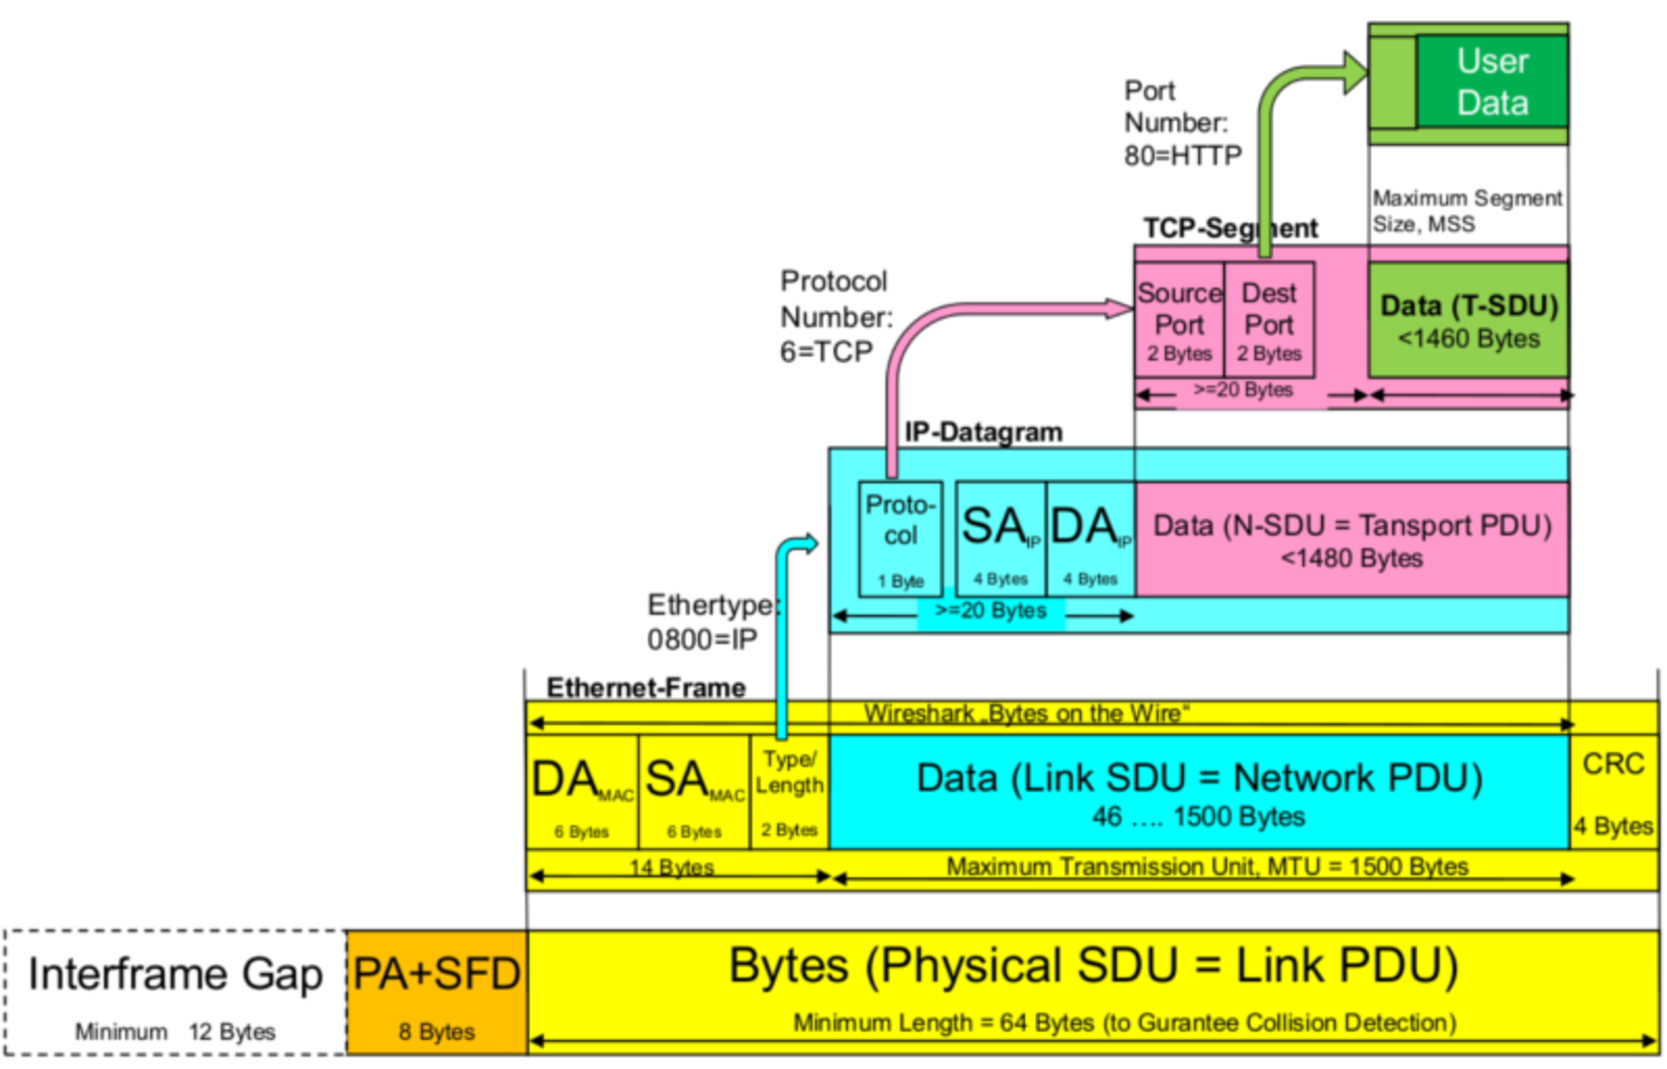
\includegraphics[width=0.7\linewidth]{images/osi_headers}
\caption{OSI Headers}
\end{figure}

\subsection{Zahlensysteme}
\subsubsection{Dezimal in Hexadezimal}	
\begin{align}
\begin{split}
	1278_D &\rightarrow Hexadezimal? \\
	1278 : 16 &= 79 \text{ Rest } 14 \Rightarrow E \\
	79 : 16 &= 4 \text{ Rest } 15 \Rightarrow F \\
	4 : 16 &= 0 \text{ Rest } 4 \Rightarrow 4 \\
	1278_D &\Rightarrow \underline{4FE}
\end{split}
\end{align}

\subsubsection{Hexadezimal in Binär}
\begin{align}
\begin{split}
	4FE_H &\rightarrow Binär? \\
	4 &= 4_D = 0100_B \\
	F &= 15_D = 1111_B \\
	E &= 14_D = 1110_B \\
	4FE_H &\Rightarrow \underline{0100 1111 1110}
\end{split}
\end{align}

\subsubsection{Hexadezimal in Dezimal}
Möchte man eine IPv6 Adresse in IPv4 umwandlen, nimmt man immer 2 Hexzahlen und rechnet diese einzeln in dezimalZahlen um
\begin{align}
\begin{split}
	0F:2049 &\rightarrow Dezimal? \\
	0_H &\Rightarrow 0_D \cdot 16^1 = 0 \\
	F_H &\Rightarrow 15_D \cdot 16^0 = 15 \\
	2_H &\Rightarrow 2_D \cdot 16^1 = 32 \\
	0_H &\Rightarrow 0_D \cdot 16^0 = 0 \\
	4_H &\Rightarrow 4_D \cdot 16^1 = 64 \\
	9_H &\Rightarrow 9_D \cdot 16^0 = 9 \\
	4FE_H &\Rightarrow (0+15) . (32 + 0) . (64 + 9) = \underline{xxx.15.32.73}
\end{split}
\end{align}

\section{Subnetting}	
\subsection{Classful}
Bei Classfull Subnetting sind alle Subnetzmasken gleich. Die Subnetzmaske ist immer so gross, wie das grösste Subnetz. \\
\begin{tabu} to \linewidth {|l|l|X|X|}
	\hline
	Klasse 	& Binär Präfix & IP-Range & Netzmaske\\ 
	\hline\hline
	A 		& 0\_\_\_.	& 0.0.0.0 - 127.255.255.255 	& 255.0.0.0  \\ 
	\hline
	B 		& 10\_\_.	& 128.0.0.0 - 191.255.255.255 	& 255.255.0.0 \\ 
	\hline
	C 		& 110\_.	&  192.0.0.0 - 223.255.255.255 	& 255.255.255.0\\ 
	\hline
	D 		& 1110.		& 224.0.0.0 - 239.255.255.255 	& Verwendung für Multicast  \\ 
	\hline
	E 		& 1111.		& 240.0.0.0 - 255.255.255.255 	& reserviert für zukünftige Zwecke  \\ 
	\hline
\end{tabu}

\subsubsection{Private Adressbereiche}
\begin{tabu} to \linewidth {|X|X|X|}
	\hline
	Klasse 	& Adressbereich & CIDR Prefix \\ 
	\hline\hline
	A		& 10.0.0.0 bis 10.255.255.255	& 10.0.0.0/8 \\ 
	\hline
	B		&  172.16.0.0 bis 172.31.255.255 		& 172.16.0.0/12 \\ 
	\hline
	C		& 192.168.0.0 bis 192.168.255.255	& 192.168.0.0/16\\ 
	\hline
\end{tabu}

\subsection{VLSM: Variable Length Subnetting /CIDR: Classless Inter-Domain Routing}
Bei Classless können flexiblere Adressgrössen verwendet werden. Dabei müssen aber trotzdem Blöcke gemäss dem grössten Subnetz gemacht werden. Diese Blöcke können aber im Gegensatz zu Classful Subnetting in kleinere Netze unterteilt werden. 

\subsection{Vorgehen}
Angenommen man bekommt  Netz 172.16.0.0/16 (Class B) und muss dieses in mehrere Subnetze unterteilen. Es empfiehlt sich immer mit dem grössten Netz (mit den meisten Hosts) zu beginnen und dann immer kleinere Subnetze zu berechnen.	
\begin{enumerate}
	\item Man sucht sich das grösse Subnetz (angenommen 634 Hosts) und berechnet dessen Subnetzmaske: 624 Hosts $\Rightarrow 2^{10} = 1024 \text{ verfügbare Hosts} \Rightarrow /22 = 255.255.252.0$ 
	\item Die Bits 16 - 22 können nun für die Subnetze genutzt werden
	\[ 1111 1111 . 1111 1111 . |0000 00|00 . 0000 0000 \]
	\[ 1111 1111 . 1111 1111 . |0000 01|00 . 0000 0000 \]
	\[ 1111 1111 . 1111 1111 . |0000 10|00 . 0000 0000 \]
	\[ 1111 1111 . 1111 1111 . |0000 11|00 . 0000 0000 \]
	\item Im Subnetz Bereich werden nun die Bits binär hochgezählt (Startend bei 0000)
	\item Die resultierenden Werte sind jeweils die Netzadressen
	\item Das 0-er Netz wird meist für die Links verwendet (/30)
	\item Beachte, dass immer zwei Adressen in jedem Subnetz für Broadcast und Netzadresse reserviert
\end{enumerate}

\subsubsection{Subnetzmasken}
\begin{tabu} to \linewidth {|l|l|}
	\hline
	CIDR 	& Subnetzmaske\\ 
	\hline\hline
	/30 & 255.255.255.252 \\ \hline
	/29 & 255.255.255.248 \\ \hline
	/28 & 255.255.255.240 \\ \hline
	/27 & 255.255.255.224 \\ \hline
	/26 & 255.255.255.192 \\ \hline
	/25 & 255.255.255.128 \\ \hline
	/24 & 255.255.255.0 \\ \hline
	/23 & 255.255.254.0 \\ \hline
	/22 & 255.255.252.0 \\ \hline
	/21 & 255.255.248.0 \\ \hline
	/20 & 255.255.240.0 \\ \hline
	/19 & 255.255.224.0 \\ \hline
	/18 & 255.255.192.0 \\ \hline
	/17 & 255.255.128.0 \\ \hline
	/16 & 255.255.0.0 \\ \hline
\end{tabu}

\subsubsection{IPv6}
Empfohle werden fixe Netze von der Grösse /64
	
\section{Cisco Command Line Interface (CLI)}

\subsection{Modes}
Cisco Router sind in Berechtigungsschichten aufgeteilt. Jeder Modus erlaubt es unterschiedliche Aktionen auszuführen. Möchte man innerhalb des Konfigurationmodus ein show Befehl ausführen muss ein "do" vor gehängt werden.
\begin{description}
	\item[Usermode] Standmodus. In diesem Modus können "public" Router Einstellungen nur betrachtet werden
	\item[Priviledge Mode] Mit 'enable' rsp. 'en' kann in den privilegierten Modus gewechselt werden. Dieser Modus erlaubt das betrachten von "privaten" Einstellungen.
	\item[Configuration Mode] Mit 'configure Terminal' rsp. 'conf t' kann in den konfigurations Modus gewechselt werden. Hier können Einstellungen im Memory konfiguriert werden.
	\item[Interface Configuration Mode] Mit 'interface' kann ein Interface Konfiguriert werden
	\item[Router Configuration Mode] Mit 'router' kann z.B das Routing Protokoll geändert werden.
\end{description}

\subsection{Konfiguration anzeigen}
\begin{tabu} to \linewidth {|X|X|}
	\hline
	Aktuelle Konfiguration filtern (Ganz Block anzeigen) 	& show run | section <my filter>\\ 
	\hline
	Aktuelle Konfiguration im RAM filtern (Zeile anzeigen) 	& show run | include <my filter> \\ 
	\hline
	Aktuelle Konfiguration im NVRAM anzeigen	& show startup-config \\ 
	\hline
	Verbundene Geräte anzeigen	& show cdp neighbor \\ 
	\hline
	Laufende Routing Protokolle anzeigen 	& show ip protocols \\ 
	\hline
	Routing Tabelle anzeigen	&  show ip route \\ 
	\hline
	Interface Übersicht anzeigen	&  show ip interface brief \\ 
	\hline
\end{tabu}

\subsection{Konsole konfigurieren}
\begin{tabu} to \linewidth {|X|X|} 
	\hline
	Konsole konfigurieren & line console 0\\ 
	\hline
	Session Timeout setzen (für die Konsole) &  	exec-timeout [min][sec] \\ 
	\hline
	Synchrones logging aktivieren & logging synchronous \\ 
	\hline
\end{tabu}

\subsection{Rooter konfigurieren}
\begin{tabu} to \linewidth {|X|X|}
	\hline
	Hostname setzen & hostname name\\ 
	\hline
	Statischen Eintrag in die Hostname Tabelle einfügen & ip host <name>\\ 
	\hline
	Passwort setzen & enable secret <my secret> \\ 
	\hline
	DNS Lookup deaktivieren (Somit werden Falscheingaben nicht aufgelöst) & no ip domain-lookup \\ 
	\hline
	IP Route leeren & clear ip route *\\ 
	\hline
\end{tabu}

\subsection{NAT konfigurieren}
\begin{tabu} to \linewidth {|X|X|}
	\hline
	NAT Tabelle eintragen & show ip nat translation \\ 
	\hline
	Statisches Port forwarding & ip nat inside source static tcp <local client> <port> interface <interface> <port> \\ 
	\hline
\end{tabu}

\subsubsection{RIP}
\begin{tabu} to \linewidth {|X|X|}
	\hline
	RIP konfigurieren & router rip \\ 
	\hline
	Welche direkt angehängte Netzerke via RIP advertised werden sollen & network <net ip> \\ 
	\hline
	Verwendete RIP Version setzen & version 2 \\ 
	\hline
	Automatisches Zusammenfassen von Netzen deaktivieren & no auto-summary \\ 
	\hline
	Mögliche Fehler der RIP Konfiguration anzeigen & debug ip rip \\ 
	\hline
\end{tabu}

\subsubsection{OSPF}
\begin{tabu} to \linewidth {|X|X|}
	\hline
	OSPF konfigurieren. Prozess ID kann beliebig gewählt werden. Gilt Router lokal & router ospf <process-id [1-65535]>\\ 
	\hline
	Welche direkt angehängte Netzerke via OSPF advertised werden sollen & network <net ip> <inverse-subnet> area <area-id> \\ 
	\hline
	Wie oft der Shortest Path Algorithmus ausgeführt wurde. Zeigt auch das Link State Update Intervall & show ip ospf \\ 
	\hline
	Zeigt die OSPF Nachbarn & show ip ospf neighbor\\ 
	\hline
	Zeigt die Topologie Datenbank & show ip ospf database \\ 
	\hline
\end{tabu}

\subsubsection{BGP}
\begin{tabu} to \linewidth {|X|X|}
	\hline
	BGP aktivieren & router bgp <as-number> \\ 
	\hline
	BGP Nachbarn eintragen & neighbor <ip-address> remote-as <as-number> \\ 
	\hline
	BGP Debuggen & debug condition interface <interface>\\
	\hline
	BGP Debuggen & debug ip packet detail\\ 
	\hline
	Alle BGP Infos anzeigen & show ip bgp\\ 
	\hline
	BGP Infos anzeigen & show ip bgp summary\\ 
	\hline
\end{tabu}

\subsection{Interface konfigurieren}
\begin{tabu} to \linewidth {|X|X|}
	\hline
	Zu konfigurierendes Interface auswählen & interface [f/g]0/1 \\ 
	\hline
	IP Konfiguration setzen & ip address <ip> <subnet mask>  \\ 
	\hline
	Beschreibung setzen & Description <description>  \\ 
	\hline
	Interface aktivieren & no shutdown  \\ 
	\hline
	Serial-Clock-Speed einstellen & clock rate 128000 \\
	\hline
\end{tabu}

\subsection{Konfiguration speichern}
\begin{tabu} to \linewidth {|X|X|}
	\hline
	Routing Konfiguration speichern & copy running-config startup-config \\ 
	\hline
\end{tabu}

\subsection{Debugging}
\begin{tabu} to \linewidth {|X|X|}
	\hline
	Debuging aktivieren & debug ip routing \\ 
	\hline
	Debuging deaktivieren & undebug all \\ 
	\hline
\end{tabu}

\subsection{Routing}
\begin{tabu} to \linewidth {|X|X|}
	\hline
	Statische Route eintragen 	& ip route <target-net> <target-subnet> <next-hop> <path-cost>\\ 
	\hline
\end{tabu}

\section{Cisco Router Komponenten}
\paragraph{DRAM: Dynamic RAM / RAM: Random Access Memory}
\begin{itemize}
	\item Routing Tabellen
	\item ARP Cache
	\item Fast Switching Cache
	\item Packet buffering
	\item Beinhaltet die Routing Konfiguration während der Router eingeschaltet ist
	\item Verliert den Inhalt sobald der Router neugestartet wird
\end{itemize}

\paragraph{NVRAM: Non Volatile Random Access Memory}
\begin{itemize}
	\item Beinhaltet die Startup und Backup Konfiguration des Routers
	\item Behält den Inhalt, auch wenn der Router abgeschalten oder neugestartet wird
\end{itemize}

\paragraph{Flash Speicher}
\begin{itemize}
	\item Beinhaltet das System Image
	\item Erlaubt das Updaten der Software ohne das der Chip auf dem Prozess ausgetauscht werden muss.	
	\item Behält den Inhalt, auch wenn der Router abgeschalten oder neugestartet wird	
	\item Kann mehrere IOS Software beinhalten
\end{itemize}

\paragraph{ROM: Read Only Memory}
\begin{itemize}
	\item Stellt Instruktionen für POST (power-on-self-test) Diagnosen zur Verfügung
	\item Speichert Bootstrap Programme und Grundlegende OS Software
	\item Benötigt ersetzbare, einsetzbare Chips für Software Updates
\end{itemize}

		
\section{Telefonie}
\subsection{Vermittlungsarten}
\begin{description}
	\item[Leitungsvermittlung (circuit switched)] \hfill \\
	Bei der Leitungsvermittlung geht der komplette Traffic über eine reservierte Leitung. Dies hat den Vorteil, dass man garantierter QoS hat, dass man das Netzwerk für eine bestimmte Funktion optimieren kann und dass es sehr stabil ist. Nachteil ist ganz klar, dass die ungenutzte Übertragungskapazität nicht für andere Services genutzt werden. Ein klassisches Beispiel für die Leitungsvermittlung ist das Telefonienetz, wobei die Signalisierung heutzutage über SS7 läuft.
	\item[Paketvermittlung (packet switched)] \hfill \\
	Bei der Paketvermittlung wird der Weg anhand der Destination Adresse des Pakets entschieden. Dadurch kann es möglich sein, dass die Pakete unterschiedlich schnell beim Empfänger ankommen. Der Vorteil bei der Paketvermittlung ist, dass es flexibler ist und die Kosten pro Datenvolumen, rsp. FlatRate anfallen.
\end{description}

\subsection{PSTN: Public Switched Telephone Network}
PSTN (früher ein Synonym für POTS: Plain Old Telephone Service $\Rightarrow$ analoges Netz) war das erste öffentliche Kommunikationssystem für die Telefonie. Es existierte eine physikalische Verbindung (Leitungsvermittlung) zwischen den Teilnehmer, wobei in der ersten Version eine Person die Verbindung manuell herstellte. In späteren Versionen wurde mittels Pulse Code Modulation das analoge Signal in ein Digitales umgewandelt.

\subsection{ISDN: Integrated Service Digital Network = PSTN IV}
ISDN lösste das analoge PSTN ab, da dieses stark limitiert war. ISDN unterstützt die Übertragung von Daten, Sprache und Video, wobei es mit einer Übertragungsrate von 64kbps für Sprachübertragung optimiert wurde. 

\subsubsection{Anschlüsse}
Ein ISDN-Anschluss ist in zwei Varianten verfügbar
\begin{description}
	\item[Basisanschuss:] Es stehen zwei B-Kanäle (Nutzkanäle) zur Verfügung, die völlig unabhängig voneinander für Telefongespräche, Fax oder Datenübertragung genutzt werden können. Zusätzlich gibt es einen D-Kanal (Steuerinformationskanal)
	\item[Primärmultiplexanschluss:] Es stehen 30 B-Kanäle und ein Steuerkanal, sowie einen weiteren Kanal für die Synchronisation und Wartung zur Verfügung.
\end{description}

\subsection{IP-Telefonie}
IP-Telefonie baut im Gegensatz zur herkömmlichen PSTN/ISDN Technologie (verbindungsoriertiert) auf ein verbindungsloses UDP Protokoll auf und sendet die einzelnen Pakete durch eine Wolke aus Switches und Router. IP-Telefonie hat dabei den klaren Vorteil, dass eine Verbindung für die Gesprächsdauer nicht fix reserviert wird und somit ungenutzte Übertragungskapazitäten für andere Teilnehmer zur Verfügung stehen.

\subsection{SIP: Session Initiation Protocol}
SIP eignet sich für den Aufbau, Betrieb und Abbau von Sprach- und Video-Verbindungen. Sowohl Punkt-zu-Punkt- als auch Multicast-Verbindungen lassen damit steuern. In der Grundversion werden die Informationen im Klartext übertragen. Da dies ein enormes Sicherheitsrisiko ist, sollte die SIPS verwendet werden.

\begin{itemize}
	\item SIP ist ein textbasiertes Protokoll dass die Verbindung zwischen zwei Teilnehmer steuert.
	\item SIP beschreibt nur die Signalisierung. Alles Weitere wird über SDP ausgehandelt. 
	\item Durch SIP wird eine verbindungsorientiert Kommunikation in einem paketvermittelnden Netz realisiert
	\item Es arbeitet auf Layer 5-7 und verwendet TCP und UDP auf Port 5060-5061
	\item Mit RTP (Real-Time Transport Protocol)  werden die Medienströme in Echtzeit übertragen. Dies geschieht jedoch unverschlüsselt! Man sollte daher SRTP verwenden. 
	\item Als Ersatz für die Telefonnummern wird ein Teilnehmer mit einer URI und DNS addressiert (sip:userid@domain)
	\item SIP verfügt über die User Location, Availability und Capabilities. 
\end{itemize}

\subsubsection{SIP Komponenten}
Eine SIP Infrastruktur kann über folgende Komponenten verfügen, wobei nur die Uesr Agents pflichts sind und ein physisches Gerät die Funktionen mehrere logischen Komponenten übernehmen.
\begin{description}
	\item[User Agent] \hfill \\
	Das Endgerät. Es wird zwischen User Agent Client (UAC) $\Rightarrow$ Caller, Sender und User Agent Server (UAS) $\Rightarrow$ Callee,Empfänger unterschieden.	
	\item[Gateway] \hfill \\ 
	Übernimmt die Übersetzung von PSTN Geräten zum SIP Protokoll. Ein Gateway ist nur eine spezielle Variante eines User Agents
	\item[Registrar] \hfill \\
	 Linked die SIP URI mit der Geräte IP Adresse. Nimmt SIP:Register Meldungen entgegen und beinhaltet alle aktuellen Standorte der UA innerhalb der Domäne.	
	\item[Proxy Server] \hfill \\
	Routet und verbindet zwei Endgeräte. Nimmt UAC Request entgegen, fragt den Registrar nach der Adresse des UAS und leitet die Verbindung weiter. Ist die Adresse auserhalb seiner zuständingen Domäne, wird der Request an einen weiteren Proxy weitergeleitet. Ein Proxy kann ein Invite auch an mehrere Endgeräte senden und verbindet dann mit jedem, welches ein OK zurücksendet. Ein SIP Proxy kann entweder stateless oder stateful sein:
	\begin{itemize}
		\item Stateless: Leitet die SIP Pakete weiter ohne über den Status bescheid zu wissen.
		\item Statefull: Verwendet immer TCP und verwaltet den Status der Verbindung bis diese terminiert wird.
	\end{itemize}
	\item[Redirect Server] \hfill \\
	Adressbuch, nimmt Anfragen entgegen und antwortet mit Adresse
\end{description}

\subsubsection{SIP Meldungen}
Das Protokoll unterscheidet zwischen Request und Responses:
\begin{description}
	\item[Request:] REGISTER (Registrier eine UA bei Registrar), INVITE, ACK, BYE, CANCEL, OPTIONS
	\item[Response:] \hfill \\
	HTTP Status Code
	\begin{itemize}
		\item 1xx = Informational
		\item 2xx = Success
		\item 3xx = Redirection
		\item 4xx = Client Error
		\item 5xx = Server Error
		\item 6xx = Global Error
	\end{itemize}
\end{description}

\subsubsection{Ablauf}
\begin{enumerate}
	\item Der Sender sendet dem Empfänger ein INVITE (kann auch über einen Proxy gehen)
	\item Der Empfänger antwortet mit einem 100(Trying), 180 (Ringing ) und Status Code 200 (OK)
	\item Der Sender antwortet mit einem ACK und die Verbindung ist aufgebaut
	\item Der UA der die Verbindung schliesst sendet ein BYE worauf die Gegenstelle mit einem Status Code 200 OK Antwortet
\end{enumerate}

\begin{figure}[h]
\centering
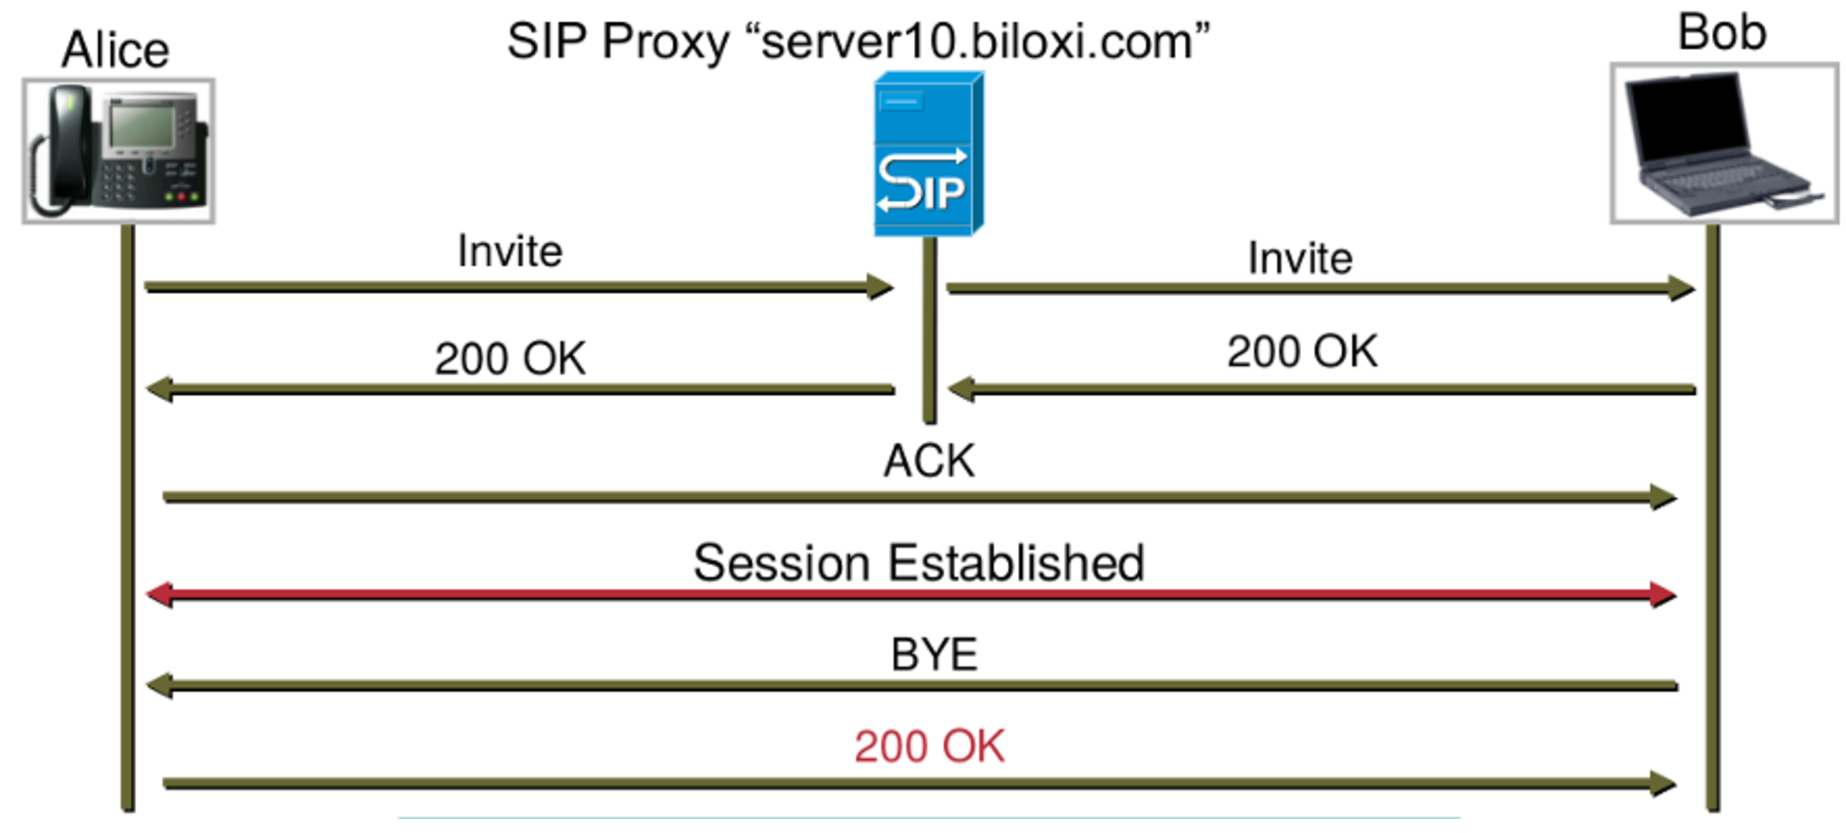
\includegraphics[width=0.7\linewidth]{images/sip_messages}
\caption{SIP Anruf Ablauf mit Proxy}
\end{figure}


\subsubsection{SDP: Session Description Protocol}
Mit SDP werden Medienbeschreibung (Video, Audio), Transportprotokoll(RTP, UDP, IP, H.320),  Codec (H.261, MPEG), Ports und Senderichtung ausgetauscht. SDP wird z.B beim SIP Invite für das Aushandeln der Codecs verwendet. SDP ist textbasiert wobei die Reihenfolge der Eigenschaften eine Rolle spielt:
\begin{enumerate}
	\item v = <protocol-version> (Pflicht)
	\item o = <username> <session-id> <session-version> <nettype> <addrtype> <unicast-address> (Pflicht)
	\item s = <session-name>
	\item c = <nettyp> <addrtype> <connection-address> (Pflicht)
	\item k = <encryption-keys>
	\item t = <time the session is active> (Pflicht)
	\item m = <media> <port> <protocol> <fmt (Link auf a Eintrag)>  (Pflicht)
	\item a = <media attribute lines> (Reihenfolge der a Einträge entsprechen deren Priorität)
\end{enumerate}

\subsection{ENUM: Telephone Number Mapping}
ENUM mappt herrkömmliche PSTN Telefonnummern mit SIP Adressen. Dies erlaubt die Kommunikation zwischen PSTN und IP-Telefonie. Dabei wird eine DNS Anfrage vom Gateway mit der umgedrehten Telefonnummer gestellt. (0.1.0.2.2.9.3.4.4.1.4.e164.arpa) Der DNS Server antwortet mit der SIP Adresse.


\section{WLAN: Wireless LAN}

\begin{description}
	\item[SSID:] Service Set Identifier
	\item[BSSID:] Basic Service Set Identifier. Meistens die MAC Adresse des Access Points
	\item[BSS:] Basic Service Set
	\item[ESS:] Extended Service Set. Mehrere BSS mit gleicher SSID
	\item[RSSI:] Received Signal Strength Indicator. Stellt einen Indikator für die Empfangsfeldstärke kabelloser Kommunikationsanwendungen dar.
	\item[CSMA/CA:] Carrier Sense, Multiple Access, Collision Avoidance
	\item[SIFS:] Short Interframe Gap. Dient dazu einen Sicherheitsabstand zwischen zwei Übertragungsblöcke einzubauen, damit sich diese nicht gegenseitig beeinflussen. SIFS hat die höchste Priorität; eine Station mit SIFS darf vor allen anderen Stationen senden. Typische SIFS-Intervalle betragen im 2,4-GHz-Frequenzband 10$\mu s$ und im 5-GHz-Band 16$\mu s$.  
	\item[DIFS:] Distributed Interframe Space. Er hat die längsten Wartezeiten mit etwa 50$\mu s$ zuzüglich dem Backoff und die geringste Priorität. 
	\item[EIFS:] Extended Interframe Space. Das EIFS kommt immer dann zum Einsatz, wenn eine Station in einem Funknetz unvollständige oder fehlerhafte Datenpakete empfängt, oder wenn die Übertragung durch die Bitübertragungsschicht abgebrochen wurde.
	\item[ACK:] Acknowledge
	\item[RTS:] Requst to Send.
	\item[CTS:] Clear to Send.
\end{description}

\subsection{Passive Mode}
\begin{itemize}
	\item Access Points versenden Beacon Frames um den Clients ihre Möglichkeiten zu übermitteln. Diese werden in regelmässigen Intervallen versendet.
\end{itemize}

\subsection{Active Mode}
\begin{enumerate}
	\item Die Clients hingegen senden Probe Requests an die Access Points um ihre Möglichkeiten bekannt zu machen
	\item Der Acces Point antwortet mit Probe Response
	\item Um die Rückwärtskompatibilität zu gewährleisten, wird nach einem erfolgreichen Probe Response ein Authentication Request und Response versendet.
	\item Danach erfolgt das Verbinden mit genau einem Access Point mittels einem Association Request und Response.
	\item Wechselt ein Client seinen Standort ist eine Reassoziierung von Nöten. (Handover) Es werden Reassociation Request und Responses versendet, falls sich der Client innerhalb eines ESS bewegt.
\end{enumerate}

\subsection{Datenrate}
\begin{itemize}
	\item Die maximal erreichbare Datenrate hängt von mehreren Kriterien ab
	\begin{enumerate}
		\item Signal bzw. Kanalbandbreite
		\item Signal zu Geräusch Verhältnis
		\item Anzahl parallel nutzbare Ausbreitungswege (MIMO)
	\end{enumerate}
\end{itemize}

\subsection{2.4Ghz Band}
\begin{itemize}
	\item IEEE 802.11b/g/n
	\item Grössere Reichweite und Kompatibilität mit Legacy Geräten
	\item Kanalbandbreite von 22Mhz
	\begin{itemize}
		\item 20Mhz: Von verfügbaren 13 Kanälen können 3 überlappungsfrei genutzt werden(meist 1, 6, 11)
	\end{itemize}
\end{itemize}

\subsection{5hz Band}
\begin{itemize}
	\item IEEE 802.11a/n/ac
	\item Geringe Reichweite dafür weniger störungsanfällig und grössere Bandbreite
	\item Kanalbandbreite kann 20, 40Mhz sein
	\begin{itemize}
		\item 20Mhz: 19 überlappungsfreie Kanäle (Kanal 36, 40, 44 .. 140)
		\item 40Mhz: 9 überlappungsfreie Kanäle
	\end{itemize}
\end{itemize}

\subsection{Antennen}
Es gibt viele WLAN-Antennen welche sich in deren Grösse und Form unterscheiden,
wobei dies einen Einfluss auf das resultierende Signal hat. Bei höheren Frequenzen werden
die Antennen kleiner, wie auch deren Reichweite.

\begin{description}
	\item[Omnidirektionale Antennen] Omnidirektionale Antennen haben eine donought-artige Abdeckung. Die Sendeleistung um die Antenne herum ist gut und sehr gleichmässig. Direkt über und unterhalb der Antenne ist die Sendeleistung am schwächsten. 
	\item[Gerichtete Antennen] Gerichtete Antennen haben konzentrieren ihre Abdeckung auf einen Punkt und sin deshalb für die Überbrückung von grösseren Distanzen geeignet.
\end{description}
 
\subsection{Sendelesitung}
\subsubsection{TPC: Transmitted Power Control}
Ist eine Regelung für die abgestrahlte Sendeleistung.

\subsubsection{Einschränkungen}
Einschränkungen werden vom BAKOM (Bundesamt für Kommunikation) vorgeschrieben und soll die Beeinträchtigung anderer Funksysteme wie die für militärische Radarsysteme oder die für die Satellitenkommunikation minimieren.
\begin{itemize}
	\item 2.4GHz Frequenzband: max. 100mW
	\item Unteres 5Ghz Frequenzband(indoor): max 200mW ohne TPC Funktionalität, ansonsten 100mW
	\item Oberes 5Ghz Frequenzband (indoor/outdoor):  max 1W (mit TPC) und 500mW (ohne TPC)
\end{itemize}

\subsection{FHSS: Frequence Hopping Spread Spectrum}
Bei FHSS wird alle paar Millisekunden die Frequenz innerhalb des Frequenzbereiches gewechselt. Dies hat den Vorteil, dass sich die Geräte weniger stören. Da während des Wechsels keine Daten übertragen werden können, leidet aber die Übertragungsrate. Es wird unter anderem bei Bluetooth eingesetzt.

\subsubsection{EIRP}
Die Equivalent Isotropically Radiated Power (EIRP) ist ein Mass für die maximale Signalstärke.
\[
	\underbrace{EIRP}_{Strahlenleistung} = \overbrace{P_T}^{Eingespeiste Leistung} - \underbrace{L_c}_\text{Verlust im Kabel} + \overbrace{G_a}^\text{Antennengewinn}
\]

Die EIRP wird in Decibel Miliwatt(dBm)  ausgedrückt:
\[
Power_{dBm} = 10 \cdot log_{10}(Power_{mW}/1mW)
\]	
	
\begin{figure}[h]
\centering
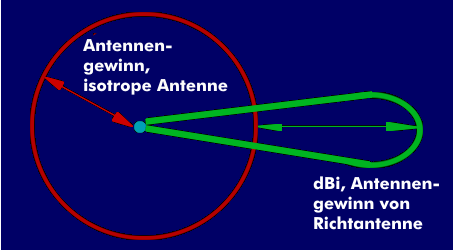
\includegraphics[width=0.5\linewidth]{images/eirp}
\caption{Effektive Isotrope Strahlungsleistung EIRP}
\label{fig:eirp}
\end{figure}

\subsection{Signal zu Rausch Verhältnis}
Das Signal-Rausch-Verhältnis (SNR) ist das Verhältnis aus der Leistung des übertragenen Nutzsignals zur Leistung des Rauschsignals und ein Maß für die Reinheit eines Signals. Je größer das Signal-Rausch-Verhältnis ist, desto störungsfreier und weniger verrauscht ist das Nutzsignal. 
\[
	SNR = 10 \cdot log_{10}(\frac{Nutzsignalleistung}{Rauschleistung}) dB
\]

\subsection{Multipath}
Unter eine Multipath versteht man die Ausbreitung von ungerichteten Funkfrequenzen. Solche ungerichtete Funkfrequenzen breiten sich beim Senden in verschiedene Richtungen aus und legen durch Beugung, Brechung, Fading und Reflexion unterschiedlich lange Wege zurück, bevor sie beim Empfänger mit unterschiedlichen Phasenlagen eintreffen. Die einzelnen Phasenlagen der Eingangsfrequenzen bilden sich am Empfängereingang als Interferenzen aus, die sich in starken Feldstärkeschwankungen bemerkbar machen. 

\subsection{MIMO: Multiple Input, Multiple Output}
Das Grundkonzept von MIMO ist Raummultiplex mit einer Vervielfachung der Funkstrecken durch Mehrwegeausbreitung. Die einzelnen Funksignale, die von einem räumlich verteilten Antennen-Array abgestrahlt werden, haben die gleichen Frequenzen und werden als Spatial Streams (SS) bezeichnet.
\begin{itemize}
	\item Unterstützt mehrere Sende- und Empfängerantennen um das Signal zu Rausch Verhältnis (SNR) zu verbessern
	\item Unterstützt das Senden mehrere Signalen zur gleichen Zeit
\end{itemize}

\subsubsection{Multi User MIMO}
Während in SU-MIMO nur ein Frame mit Zieladresse an einen einzelnen WLAN-Client übertragen werden kann, können in MU-MIMO gleichzeitig mehrere Frames mit unterschiedlichen Zieladressen an mehrere individuelle WLAN-Clients übertragen werden. 
\begin{itemize}
	\item Wird unterstützt ab 802.11ac
\end{itemize}

\subsection{Channel Bonding}
Channel Bonding beschreibt das Zusammenlegen mehrere Kanäle in einen grösseren um die Kanalbandbreite zu erhöhen.

\subsection{Packet Aggregation}
Bei Packet Aggregation werden mehrere Pakete in ein Frame verpackt, damit der Overhead minimiert werden kann.

\subsection{Cisco Client Link}
Diese Technologie dient zur Überbrückung der Abdeckungslücken von Access Points, die auf unterschiedliche Clients (802.11a/g/n und ac) zurückzuführen sind. Sie verbessert die Zugriffsleistung und Reichweite sowie die Benutzerfreundlichkeit des Wireless-Netzwerks.
	
\subsection{IAPP: Inter Access Point Protocol}
Ist ein Protokoll zur herstellerübergreifenden Kommunikation zwischen Access Points. Die Kommunikation der Access Points erfolgt per Multicast.
	
\subsection{LWAPP: Lightweight Access Point Protocol}
Ist ein Protokoll welches es erlaubt, mehrere Access Points auf einmal zu konfigurieren. Dabei gibt es einen WLAN Controller der die Konfiguration Frames auf die anderen Access Points verteilt. Der Einsatz eines Controllers bietet zudem den Vorteil, dass sich alle Clients zuerst ihm Autorisieren und somit eine unterbrechungsfreies Roaming möglich ist.

\begin{figure}
\centering
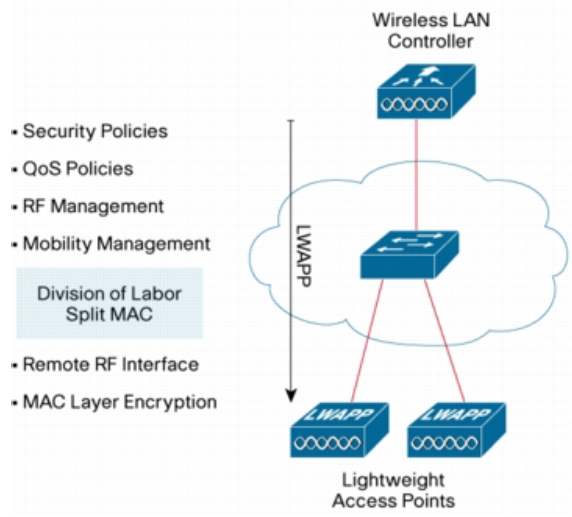
\includegraphics[width=0.5\linewidth]{images/lwapp}
\caption{LWAPP}
\end{figure}

		
\section{Switching}	
\subsection{Spanning Tree Protokolle (STP, RSTP)}
\begin{itemize}
	\item Wird eingesetzt um Broadcast Storms zu unterbinden. Layer 2 Loops werden aufgelöst.
	\item Unter RSTP werden im Gegensatz zu STP nicht nur BPDU versendet wenn solche auf dem Root Port empfangen werden, sondern alle n-Sekunden gemäss der Hello-Time. (default 2s)
	\item Werden unter RSTP 3 BPDU nicht mehr empfangen, wird die gegenüberliegende Bridge als offline betrachtet.
	\item RSTP ist rückwärtskompatibel
\end{itemize}
\subsubsection{Begriffe}
\begin{description}
	\item[STP] Spanning Tree Protocol
	\item[RSTP] Rapid Spanning Tree Protocol
	\item[BPDU] \hfill \\
		Bridge Protocol Data Unit
	\item[Root Port] \hfill \\
		Der Port mit dem kürzesten Weg zur Root Bridge. Die Root Bridge selbst besitzt keine Root Ports ist jedoch zuständig für die angeschlossenen Segmente und versendet daher die BPDU für die angeschlossenen Segmente.
	\item[Designated Port] \hfill \\
		Der zuständige Port für ein Segment
	\item[Bridge ID] \hfill \\
		8 Oktett = 2 Oktett Priorität + 6 Oktett MAC-Adresse
\end{description}

\subsubsection{Ablauf}
Spanning Trees werden immer pro VLAN aufgebaut. Grundlegend geschieht dies jedoch gemäss folgendem Ablauf:
\begin{enumerate}
	\item Auswahl einer Root-Bridge (kleinste Bridge ID)
		\begin{enumerate}
			\item jede Bridge hat alle Port im Blocking Mode
			\item jede Bridge geht davon aus selber Root Bridge zu sein
			\item versendete Configurations-BPDU mit Root-Path Kosten = 0
		\end{enumerate}
	\item Kürzesten Weg zur Root Bridge berechnen
		\begin{enumerate}
			\item Aufsummieren der Path Costs in Richtung Root Bridge
			\item Kosten sind in der Regel von der Interface Geschwindigkeit abhängig
		\end{enumerate}
	\item Für jedes Segment wird die Designated Bridge ausgewählt
		\begin{enumerate}
			\item Die Designated Bridge ist die Bridge mit den geringeren Kosten zur Root Bridge
		\end{enumerate}
	\item Root Ports werden gesetzt
		\begin{enumerate}
			\item Port mit kürzestem Weg zur Root Bridge sind Root Ports
		\end{enumerate}
	\item Alle anderen Ports gehen in den Blocking Mode
\end{enumerate}

\subsection{Virtual LAN (VLAN)}
\subsubsection{Begriffe}
\begin{description}
	\item[Trunk Port]\hfill \\ 
	Leitet den Verkehr mehrerer VLAN durch (tagged)
	\item[Access Port] \hfill \\
	Leitet den Verkehr von genau einem VLAN durch (untagged)
	\item[Native VLAN] \hfill \\
	Frames ohne Tag werden standardmässig über das Nativ VLAN übertragen. Dieses ist per default das VLAN1
	
\end{description}
\begin{itemize}
	\item Logische Workgroups innerhalb eines Netzes, auch wenn die Teilnehmer nicht physisch am gleichen Netz angeschlossen sind.
	\item VLAN ID's werden in der VLAN Datenbank abgelegt (show vlan)
	\begin{itemize}
		\item 1 - 1005: Normal Range
		\item 1005+ = Extended Range
	\end{itemize}
\end{itemize}

\subsection{VLAN Trunking Protocol (VTP)}
\begin{itemize}
	\item Arbeitet auf Layer 2
	\item Überwacht die VLAN Konsistenz
	\item Managed das Hinzufügen, Löschen und Umbenennen von VLAN innerhalb eines Netzwerks.
	\item Erkennt Misskonfigurationen
	\item Änderungen an einem Switch werden an alle anderen propagiert. (ACHTUNG: Switch mit höchster Configuration Revision Number gilt als Master Konfiguration. Hat der neue Switch die höchste Nummer, wird dessen default Config an alle anderen Switches verteilt)
\end{itemize}

\section{Routing}
\subsection{Grundlagen}
\begin{itemize}
	\item Routing kann allgemein als den Prozess des Weiterleitens eines Pakets bezeichnet werden. Router schauen dabei nur auf den Netzteil einer IP-Adresse.
	\item Für die Kommunikation zwischen zwei autonomen Systemen (AS) werden Routing Protokolle wie BGP eingesetzt. (Internet $\Rightarrow$ EGP: Exterior Gateway Protocols)
	\item Für die Kommunikation innerhalb eines autonomen Systems (AS) werden Routing Protokolle wie OSPF, EIGRP, IS-IS und älteren Netzen RIP, IGRP eingesetzt (Intranet $\Rightarrow$ IGP: Interior Gateway Protocols)
	\item Ein Routing Protokoll muss stehts über die Erreichbarkeit andere Router informiert sein. Zudem soll es den optimalen Weg zu einem Netzwerk finden und Änderungen im Netzwerk erkennen und die nötigen Anpassungen vornehmen.
\end{itemize}

\subsection{Routing Tabellen}
Pakete die an unbekannte Netzte gerichtet sind, werden per default einfach verworfen. Deshalb wird meistens als letzter Eintrag eine Default Route (0.0.0.0/0) eingetragen. Liegen mehrere Netze hinter einem Router werden diese meist in einem generischen Eintrag zusammengefasst. Ebenfalls können zwei Routen zum selben Ziel mit den gleichen Kosten eingetragen werden, um die Last auf den beiden physikalischen Verbindungen zu verteilen.
\begin{lstlisting}
R	172.16.8.0	[100/118654]	via 172.16.7.9,	00:00:23,	Serial0 \end{lstlisting}	
\begin{enumerate}
	\item Wie wurde der Eintrag gelernt (Statisch, Routing Protokoll)
	\item Zielnetz
	\item administrative Distanz / metrische Distanz
	\item Next Hop
	\item Alter des Eintrages (Stunden:Minuten:Sekunden)
	\item Interface auf welchem das Paket raus soll
\end{enumerate}

\subsection{Static Routing}
Eine statische Route wird auf einem Cisco Router wie folgt eingetragen.
\begin{lstlisting}
ip route <net address> <subnetmask> <next hop> [<costs>]\end{lstlisting}	
\subsubsection{Vorteile}
\begin{itemize}
	\item Keine unnötigen Routing Updates die das Netz belasten
	\item Sicherer, da Pakete on the Wire nicht geändert werden können
\end{itemize}

\subsubsection{Nachteile}
\begin{itemize}
	\item Statische Tabellen können sehr zeitintensiv beim Installieren / Warten sein
	\item Topologieänderungen müssen manuell umgesetzt werden. Somit kann es passieren, dass bei eienm Netzausfall solange kein Traffic fliesst, bis jemand manuell eine neue Route eingetragen hat.
\end{itemize}

\subsubsection{Default Routen}
Damit nicht zu viele Routen eingetragen werden müssen, macht man insbesondere auf Router die am Rande eines Netzwerkes stehen, sogenannte Default Routen 
\begin{lstlisting}
ip	route	0.0.0.0	0.0.0.0	192.168.98.1 \end{lstlisting}	

\subsubsection{Summary Routes}
Mit Summary Routen können mehrere Routen mit einer grösseren Subnetzmaske zusammengefasst werden.
\begin{lstlisting}
ip route 192.168.10.0 255.255.255.128 10.10.10.1
ip route 192.168.10.128 255.255.255.128 10.10.10.1

ip route 192.168.10.0 255.255.255.0 10.10.10.1
\end{lstlisting}

\subsubsection{Alternative Routen}
Alternative Routen werdne als Backup verwendet, falls eine Verbindung ausfällt. Dazu erstellt man eine alternative Route mit erhöhten Kosten, welche im normalfall nicht gewählt wird.
\begin{lstlisting}
ip route 10.1.9.0 255.255.255.0 192.168.128.33
ip route 10.1.9.0 255.255.255.0 192.168.96.1  	50	
\end{lstlisting}

\subsubsection{Load Sharing}
Um einen Lastausgleich für eine Verbindung zwischen zwei Router zu erziehlen, werden zwei Routen mit den gleichen Kosten eingetragen. Der Unterschied liegt beim Next Hop.
\begin{lstlisting}
ip route 10.1.5.0	255.255.255.0	10.1.6.2	
ip route 10.1.5.0	255.255.255.0	10.1.7.2	
\end{lstlisting}	
	


\subsection{Dynamic Routing Protokolle}
\subsubsection{Grundlegendes}
\begin{itemize}
	\item Dynamisches Routing basiert darauf, dass jeder Router seine eigene Routing-Tabelle verwaltet und in regelmässigen Abständen sein Wissen an andere Router übermittelt. Natürlich muss ein Router auch auf Informationen von anderen Geräten reagieren können. Das Routing-Protokoll berechnet dabei überall den besten Weg zu einem anderen Netzwerk.
	\item Zuerst erkennt ein Router seine lokal angeschlossenen Netze. Diese trägt er in seine Routing-Tabelle ein und übermittelt sein Wissen anschliessend an die anderen Geräte. Währenddessen erhält er Informationen von den anderen Router und trägt diese ebenfalls in seine Routing Tabelle ein.
	\item Die Kosten werden in Hops, virtuelle Kosten, Bandbreite oder Delay gemessen
\end{itemize}

\subsubsection{Distance Vector Protocol}
\begin{itemize}
	\item Ein Distance Routing Protokoll berechnet den schnellsten Weg anhand von Informationen, welch ihm seine direkten Nachbarn mitgeteilt haben. Ein Router weiss wie weit ein anderer Router entfernt ist. Generell lässt sich ein Distance Vector Protokoll mit einem Wegweiser vergleichen. Der Router kennt immer nur den nächsten Schritt/Router, ohne jedoch das Ganze, die Karte/Topologie, zu sehen.
	\item Routing by Rumor: Ein Router muss sich auf die empfangen Information verlassen und kann diese nicht auf ihre Korrektheit prüfen.
	\item Gibt es eine Änderung im Netzwerk, wird die gesamte Routing Tabelle an alle Nachbarn verteilt. (RIPv1)
\end{itemize}

\paragraph{Nachteile}
\begin{itemize}
	\item Router versenden ihre komplette Distanztabelle alle 10-90 Sekunden. Dies verursächt einen beachtlichen Netzwerktraffic in grossen Netzwerken.
\end{itemize}

\subsubsection{RIP: Routing Information Protocol}
\begin{itemize}
	\item Ist ein Routing Protokoll für das Intranet. RIP gehört zu den Interior Gateway Protocols (IGP) und ist technisch von OSPF abgelöst worden. Trotzdem wird RIP noch heute eingesetzt.
	\item RIPv1 unterstütz nur Classfull Routing. Erst ab RIPv2 wurde Classless Routing eingeführt
	\item RIP berechnet seine den besten Weg über die Hop Counts.	
\end{itemize}

\paragraph{Berechnung / Distanz Vector Algorithmus}
\[
	D^{X}(Y, Z) = \text{Distanz von X nach Y via Z} 
\]

\begin{enumerate}
	\item Mittels obiger Formel rechnet jeder Router eine Distanztabelle zu  allen anderen Router aus
	\item Anhand der Distanztabelle wird dann die Routing Tabelle abgeleitet. Dabei wird einfach der Weg mit den geringsten Kosten genommen.
\end{enumerate}

\begin{figure}[h]
\centering
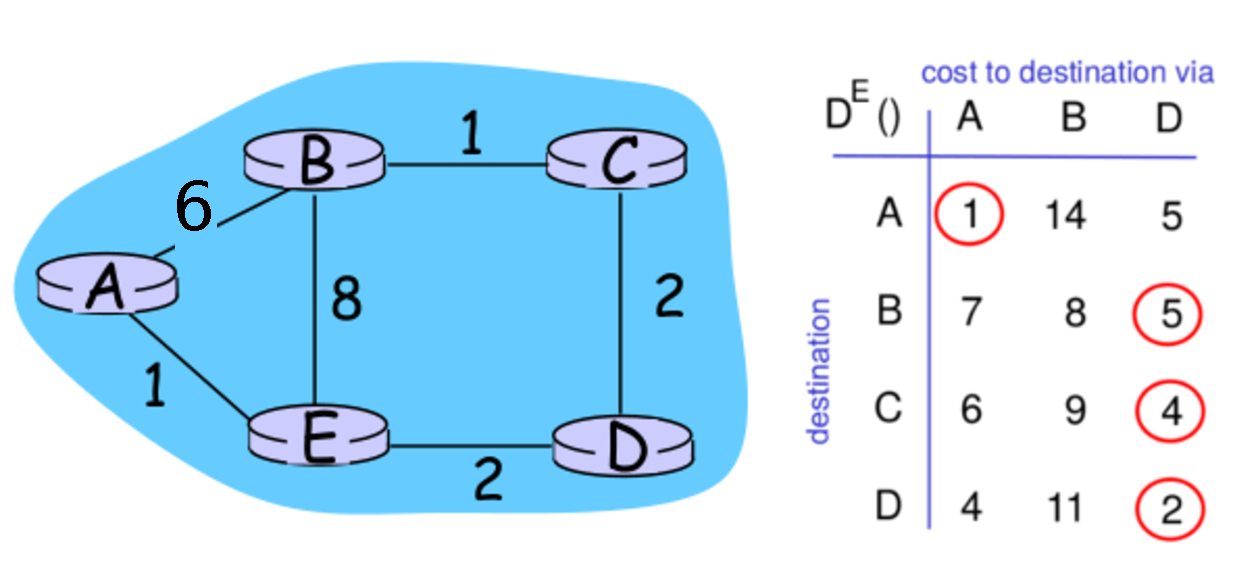
\includegraphics[width=0.7\linewidth]{images/rip}
\caption{RIP Distanz Tabelle}
\end{figure}

\paragraph{Üblicher Ablauf}
\begin{enumerate}
	\item Beim Starten eines Routers kennt dieser nur seine direkt angeschlossenen Netzwerke.
	\item Der Router trägt die Kosten zu den direkt angeschlossenen Router in seine Distanztabelle ein.
	\item Die Kosten zu einem Router der über einen anderen erreichbar ist, wird vorerst als Infinity eingetragen.
	\item Der Router erzeugt aus der Distanztabelle seine Routing Tabelle und sendet diese an seine Nachbarn.
	\item Mit den erhaltenen Informationen erweitert er seine Distanztabelle und errechnet damit eine neue Routing Tabelle.
	\item Ändern sich die minimalen Kosten, zu denen ein Router erreicht werden kann, wird wieder Schritt 2 ausgeführt.
	\item Schlussendlich hat dann jeder die selbe Routing Tabelle.
\end{enumerate}

\paragraph{Probleme}
\begin{description} 
	\item[Count-To-Infinity] \hfill \\
	Ist das Problem unendlichen hochzählens der Pfadkosten. Folgendes Beispiel sollte das Problem näher erklären.
	\begin{figure}[h]
		\centering
		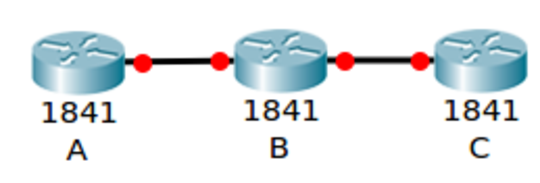
\includegraphics[width=0.3\linewidth]{images/rip_counting_infinity}
		\caption{Counting-To-Infinity}
	\end{figure}
	\begin{itemize}
		\item In einem Netzwerk mit den Routern A-B-C
		\item C geht offline
		\item B markiert C als Offline in seiner Routing Tabelle
		\item A versendet seine Routing Tabelle mit der Information, dass es C über B erreichen werden kann.
		\item B updated seine Routing Tabelle mit dieser Information und weiss dabei nicht, dass der Pfad über sich selber geht
		\item B veröffentlicht nun, dass er einen neue Weg nach C gefunden hat.
		\item Mit der neuen Information von B updated A seine Kosten nach C mit den Kosten die er von B erfahren hat. Diese beinhalten aber bereits eine Loop
		\item Die neuen Kosten propagiert A dann wieder nach B
		\item Der Prozess wiederholt sich bis ins Unendliche.
	\end{itemize}
\end{description}

\paragraph{Lösungen}
\begin{description} 
	\item[Split Horizon] \hfill \\
	Eine Pfadinformation darf nicht über dasselbe Interface veröffentlicht werden, worüber sie empfangen wurde.
	\item[Poison Reverse]\hfill \\
	Wenn der Router A eine neue Route von Router B gelernt hat, veröffentlicht er die Route zurück zu B mit einer Metrik von 16. Damit bekommt Router B nie den Eindruck, dass Router A eine bessere Route zu C kennt.	
	\item[Triggered Updates] \hfill \\
	Wenn ein Router eine Änderung in seiner Routing Tabelle detektiert, sendet er sofort (ohne das Update Intervall abzuwarten) ein "Triggered Update". Triggered Updates sind eine Möglichkeit zum ein Count-To-Infinity zu vermeiden.
	\item[Holddown Timers] \hfill \\
	Die Routen werden nicht direkt gelöscht, wenn eine Route als nicht erreichbar detektiert wird. Die Route wird vorerst mit den Kosten von 16 veröffentlicht. Dies führt dazu, dass die Nachbarn über Trigged Updates direkt über den potentiell unerreichbaren Router informiert werden. Damit werden kurze Netzausfälle überbrückt und zu grosser Routing Traffic vermieden. Nach Ablauf des Holddown Timers wird die neue Information übernommen. Neue Informationen werden angenommen und gewartet ob sich die Information bestätigt. (Default 3x30s = 90s) Der Timer wird nur bei schlechten Informationen gestartet. (grössere Kosten) Kommt währende dem Ablauf des Timers eine gute Nachricht, wird der Timer gelöscht.
	\item[Request Message] \hfill \\
	Erlaubt einem neuen Router schnell an die Routing Tabellen seiner Nachbarn zu gelangen.
\end{description}


\subsubsection{Link State Protocols}
\begin{itemize}
	\item Beim Link State Protokollen weiss ein Router über die ganze Topoligie des Netzes bescheid.
	\item Link State Protokolle sind zuverlässiger, einfacher zu debuggen und benutzen weniger Bandbreite als Distance Vector Protokolle. Dafür brauchen Link State Protokolle mehr Speicherplatz (Topologie Datenbank und Routing Tabelle) und CPU Leistung. ACHTUNG: Initial belasten LSP das Netzwerk mehr wie DVP. (Flooding von LSA)
	\item LSA = Link State Advertisement werden benötigt um Änderungen an der Topology an alle anderen Router zu propagieren.
	\item Link State Protokolle verteilen im Gegensatz zu Distance Vector Protokollen nie die ganze Routing Tabelle, sondern immer nur einzelne Einträge, die sich geändert haben.
\end{itemize}

\begin{description}
	\item[Hello Protocol] \hfill \\
	Im ersten Schritt lernen alle Router nur ihre Nachbargeräte kennen. Über Keep-Alive Nachrichten (alle 10s) wird sichergestellt, dass der Nachbar noch eingeschaltet ist. Antwortet eine Gegenstelle für 30-40s nicht mehr, wird sie als Down markiert. Für alle diese Funktion wird das Hello Protocol verwendet. Zusätzlich ist das Hello Protocol für die Parameter Aushandlung sowie für die Wahl eines Designated Routers und Backup Designated Router zuständig.
	\item[LSA: Link State Advertisements] \hfill \\
	Bei Änderungen in der Topologie informiert ein Router alle seine Nachbarn über diese Änderungen mittels LSA, welche als Trippel aus [Router\_ID, Neighbor\_ID, Kosten] bestehen. Jedes erhaltene LSA wird dabei auf allen ausgehenden Interfaces weitergeleitet und in der eigenen Datenbank abgelegt. Ein eingehendes LSA wird nie auf dem gleichen Interface veröffentlich, auf dem es reingekommen ist. Damit das Flooden nicht unendlich lange dauert, gibt es Sequenznummern innerhalb des LSA. Bereits erhaltene LSA werden nicht mehr weiter geleitet. Eine Sequenznummer ist 32Bit gross. Wird ein Router neu gestartet sendet er LSA mit der Sequenznummer 0, worauf die benachbarten Router ein LSA mit seiner letzten Sequenznummer senden.
	\item[Topologie Datenbank] \hfill \\
	Alle gesammelten Informationen aus den LSA werden in der Topologie Datenbank abgespeichert. Die Topologie Datenbank beinhaltet alle Routen zu eine Ziel, wohingegen die Routing Table nur die "besten" Routen zum Ziel speichert.
	\item[Kürzesten Pfad berechnen] \hfill \\
	Nachdem alle Tabellen verteilt wurden können die Kosten auf jedem Router berechnet werden. Dazu wird mittels Dijkstras Algorithmus ein Baum mit minimaler Länge berechnet. 
\end{description}

\subsubsection{Dijkstras Algorithmus / Shortest Path First}
\begin{enumerate}
	\item Alle Router initialisieren sich selber als Root und fügt sich mit den Kosten 0 in den Tree ein.
	\item Von dem Router, welcher zuletzt dem Tree hinzugefügt wurde, werden alle direkten Nachbarn mit den jeweiligen Kosten in Form eines Trippels	<FROM\_ROUTER>, <TO\_ROUTER>, <COST> in die Kandidatenliste geschrieben
	\subitem Ist das Ziel eines Kandidaten bereits im Baum oder ist gibt einen anderen Kandidaten mit gleichem Ziel, aber geringeren Kosten, wird der Kandidat gestrichen.
	\item Danach werden die Kosten kumuliert, von der Root aus berechnet.
	\item Die kürzeste Variante der berechneten Kosten wird dem Tree hinzugefügt. Achtung: Die Kosten im Tree entsprechen nicht den kumulierten Kosten sondern den Kosten von Router A nach Router B. 
	\item Alle übrigen Kandidaten werden für die nächste Iteration übernommen.
	\item Zu guter Letzt wird wieder bei Schritt 2 begonnen, jedoch ist der Zielrouter der zuletzt zum Tree hinzugefügten Variante der neue Ursprung. Es werden nun alle Kandidaten für diesen Router aufgelistet.
	\item Ist nur noch ein Kandidat übrig, wird dieser ebenfalls noch dem Tree hinzugefügt
\end{enumerate}
\begin{figure}[h]
\centering
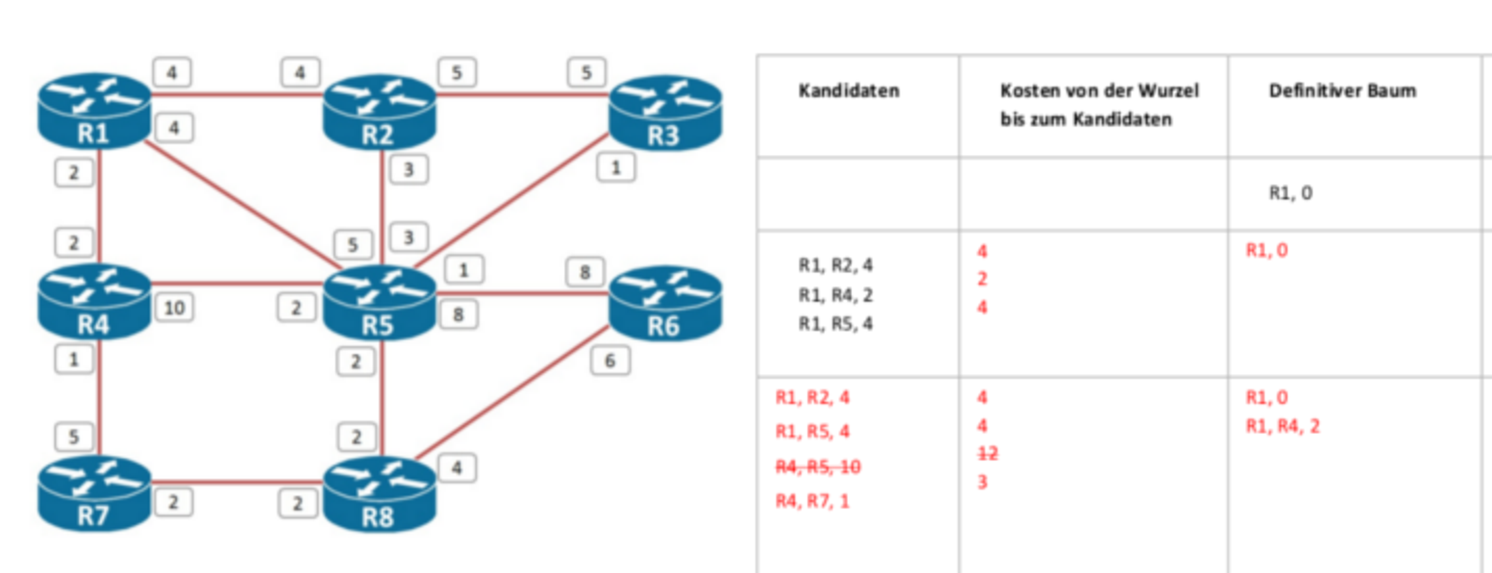
\includegraphics[width=0.7\linewidth]{images/dijkstra}
\caption{Dijkstras Tree von R1}
\end{figure}


\subsubsection{OSPF: Open Shortest Path First}
\begin{itemize}
	\item OSPF nutzt als Metrik die Bandbreite und das Delay (RIP: Hop Counts)
	\item Gibt es eine Änderung im Netzwerk, werden nur die Änderungen an die Nachbarn verteilt.
	\item Ist ein Routing Protokoll für das Intranet
	\item Implementiert das Hello Protocol, LSA und Dijkstra
	\item OSPF Pakete haben die IP Adresse 224.0.0.5 und MAC: 01-00-5e-00-00-05 (ACHTUNG: Multicast Overlapping)
	\item Bündelt Netze in sogenannte Areas damit das Verteilen einer Topologieänderung nicht zu lange dauert. Das Aufteilen in Areas hat den Vorteil dass die Routing Tabellen kleiner werden und der Rechenaufwand für den SPF Algorithmus geringer wird.
	\subitem Ein Router innerhalb der Area kennt nur die Router in seiner Area
	\subitem Ein Area Border Router (ABR) kennt die Router beider Areas zwischen welchen er routet und hat zwei Topologie Datenbanken (eine pro Area)
	\item Area 0 ist die Backbone Area
	\item Ein Netz kann mit CLI mittels folgendem Command publiziert werden: (ACHTUNG: Inverse Subnetzmaske verwenden)
	\begin{lstlisting}
	Router# network <Netzadresse> <Inverse Subnetz-Maske> area <Area-Nummer>\end{lstlisting}	
\end{itemize}

\subsection{BGP: Border Gateway Protocol}
Das Internet besteht aus autonomen Systemem (AS). Innerhalb eines AS kann jeder Betreiber seine eigenen Routing Regeln umsetzen. Jedes AS besitzt eine eigene Nummer zwischen 1 und 65535. Die oberen Nummern sind dabei für den privaten Gebrauch bestimmt. (64512-65535) Die einzelnen AS sind über BGP verbunden. 

\paragraph{Grundlagen}
\begin{itemize}
	\item TCP Port 179
	\item Path Vector Protocol mit inkrementellen Updates darüber in welchem AS eine IP-Adresse gefunden werden kann.
	\item Es gibt zwei verschiedenen Tabellen
	\begin{enumerate}
		\item In der BGP Tabelle sind alle Pfade gespeichert (show ip bgp)
		\item In der Routing Tabelle werden die besten Pfade gespeichert
	\end{enumerate} 
	\item Seit BGP4 wird CIDR unterstützt
	\item Es gibt vier verschiedene Nachrichtentypen
	\begin{enumerate}
		\item OPEN MESSAGE: Verbindungsaufbau. Neue BGP Session wird geöffent
		\item KEEPALIVE: Session erhalten, wenn keine Updates kommen
		\item UPDATES: Beinhaltet das Routing Update. Initial wird die ganze BGP Tabelle versendet, danach nur noch inkrementelle Updates.
		\item NOTIFICATION: Fehlermeldungen werden hiermit verbreitet.
	\end{enumerate}
	\item Standardverhalten
	\begin{enumerate}
		\item Interne Netzwerke werden an andere AS nach aussen propagiert
		\item Netzwerke die von anderen AS kommen, werden gelernt und weitergegeben. Dabei wird die eigene AS Nummer dem AS Pfad angehängt.
	\end{enumerate}
\end{itemize}

\subsubsection{AS: Autonomes System} Ist ein unabhängiges Netzwerk, welches von einer einzigen Organisation verwaltet wird. Dies kann eine grosse Firma oder ein ISP sein. Innerhalb eines AS wird ein einheitliches Routing Protokoll eingesetzt, welches von der Organisation bestimmt wird. Damit Informationen zwischen zwei AS ausgetauscht werden können, muss ein EGP (Exterior Gateway Protocol) wie BGP eingesetzt werden. Um BGP einzusetzen benötigt ein Unternehmen eine AS Nummer. 

\subsubsection{Single Homed AS / Ein Standort}
Um einen Standort mit dem Internet zu verbinden gibt es drei Varianten: 
\begin{enumerate}
	\item Die einfachste Variante ist die Verbindung zwischen Standort und ISP mittels statischen Routen zu verbinden
	\item Eine weitere Variante ist es, dass ein Standort seine interne Netzstruktur via OSPF dem ISP bekannt macht
	\item Eine letzte Variante ist es, dem Standort eine private AS-Nummer zu vergeben. 
\end{enumerate}

\subsubsection{Multi Homed AS / Mehrere Standorte}
Hierzu erfolgt die Anbindung ans Internet über mindestens zwei ISP's. Fällt einer der Internetprovider aus, so schaltet der Router automatisch alle Routen, die bisher über diesen liefen, auf die anderen Provider um.

\subsubsection{AS-Pfad}
Der AS Pfad besteht aus den AS Nummern welche von $AS_1$ zu $AS_n$ durchlaufen werden. Wird eine Loop detektiert wird das Update ignoriert.

\paragraph{IP Prefix} Der IP Prefix wird dem AS Pfad vorgehängt.

\subsubsection{Upstream und Downstream AS}
Upstream AS sind Netzte welche ein AS mit dem Rest der Welt verbinden. (Provider) Downstream AS sind AS welche an ein AS angeschlossen sind. (Kunden)

\subsubsection{Peering und Transit}
Unter Peering versteht man den Zusammenschluss, bzw. Weiterleitung von Daten zwischen verschieden Provider. Diese Verbindung werden mittels Verträge geregelt. In der Schweiz ist der grösste "Peering Point" das TIX in Zürich. Ein Peering Point ist ein Ort wo der Datenverkehr direkt von einem AS an ein andere übergeben wird, damit der Verkehr nicht über einen teureren upstream Provider gesendet werden muss.

\paragraph{Transit}
Transit ist spezielle eine Art von Peering. Dabei bietet ein meist sehr grosser Provider eine Verbindung zu mehreren Zielorten. Dieser Dienst ist Kostenpflichtig

\subsubsection{HSRP: Hot Standby Router Protocol}
Mehrere pyhsische Router werden zu einer logischen Gruppe zusammen gefasst. Die Gruppe von Router präsentiert sich im Netzwerk dann als ein logischer Router. HSRP wird zur Steigerung der Verfügbarkeit eingesetzt.

\subsubsection{Redistribution}
Man versteht unter Redistribution der Austausch von Routing Tabellen zwischen einem Interior und einem Exterior Routing Protokoll. 	

\subsection{NAT: Network Address Translation}
NAT wird verwendet um lokale Netzwerke mit dem Internet zu verbinden. Lokale IP-Adressen haben keine Gültigkeit im Internet. Der Einsatz von NAT resultierte aus der Adressknappheit von IPv4 Adressen. Der Router schreibt bei ausgehenden Verbindungen seine öffentliche Adresse in den IP Header und merkt sich welche TCP Verbindung zu welchem Client gehört, damit er die Antwortpakete wieder dem richtigen Client zuordnen kann.

\begin{description}
	\item[DNAT: Destination NAT] Mit DNAT können mehrere Dienste unter einer IP angeboten werden (Port Forwarding)
	\item [PAT: Port Address Translation] Zusätzlich zur IP-Adresse wird auch der Port in die Tabelle geschrieben.
\end{description}

\subsubsection{Adresstypen}
\begin{description}
	\item[Inside Local Address] Private IP-Adresse die dem Client zugeordnet ist
	\item[Inside Global Address] Öffentliche IP-Adresse des Routers
	\item[Outside Local Address] Die IP Adresse eines öffentlichen Hosts wie er im inneren Netz erscheint. Kann gleich wie die Outside Global Adresse sein, muss es aber nicht, da diese beim Router noch umgesetzt werden kann.
	\item[Outside Global Address] Die IP Adresse eines öffentlichen Hosts wie er spätestens nach dem Router erscheint. (zB. Google 8.8.8.8)
\end{description}
\begin{figure}[h]
\centering
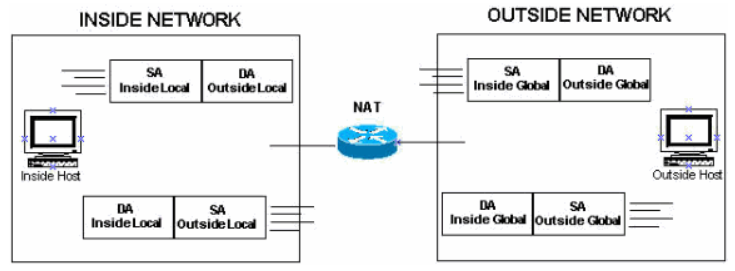
\includegraphics[width=0.7\linewidth]{images/nat_addresses}
\caption{NAT Local und Global Adressen}
\label{fig:nataddresses}
\end{figure}


\section{Multicasting}
Multicasting ist, wenn genau ein Sender IP Datagramme an eine Gruppe von Empfänger versendet. (immer via UDP) Multicast kann im Gegensatz zu Unicast Überlastungen im Netz dadurch reduzieren, dass die IP-Datenpakete nicht einzeln zwischen dem Absender und vielen Empfängern verschickt werden, sondern nur einmal zielgerichtet an alle Teilnehmer gehen. Im Gegensatz zu Unicast ist die Destination Adresse nicht die Adresse des Empfängers sonder einer ganzen Multicast Gruppe. 

\subsection{Multicast Szenarien}
\begin{description}
	\item[One-to-May] Video/Audio Broadcasts, Stocks, Software Verteilung
	\item[Man-to-May] Multicast Konferenzen, Chat Gruppen
	\item[Many-to-One] Auktionen, Abstimmungen/Wahlen
\end{description}


\subsection{Adressierung}
\begin{itemize}
	\item IPv4: 224.0.0.0 bis zu 239.255.255.255 (Klasse D, Begin mit 1110)
	\begin{itemize}
		\item Privater Bereich (Link Local): 224.0.0.0 - 224.0.0.255
		\item Globaler Bereich: 224.0.1.0 - 238.255.255.255
		\item Administrativer Bereich: 239.0.0.0 - 239.255.255.255
	\end{itemize}
	\item IPv6: FF00::/8
	\item Pseudo MAC (PMAC): 01-00-5e-00-00-00 bis 01-00-5e-7f-ff-ff
	\begin{itemize}
		\item Die letzten 23 Bits der IP Multicast Adresse wird für die letzten drei Blöcke der MAC Adresse verwendet (01-00-5e-xx-xx-xx)
		\item ACHTUNG: 	Die ersten 5Bit der IP Multicast Adresse werden nicht beachtet, was dazu führt, dass mehrere IP Adressen ($2^5 = 32$) auf die gleiche MAC Adresse führen.
		\item Die MAC Adresse verfügt über 48Bits. Dabei sind 25 fix und die restlichen 23 kommen von der IP Adresse	
	\end{itemize}
\end{itemize}

\subsection{IGMP: Internet Group Management Protocol}
Mittels IGMP, welches auf Layer 2 angesiedelt ist, kann sich ein Client für eine Multicast Gruppe bei seinem Default Gateway anmelden. Der Router sendet dann regelmässig Anfragen an 224.0.0.1 (Broadcast) ob die Mitglieder einer Gruppe immer noch Mitglieder sein wollen. Seit v2 muss sich ein Client aktiv von einer Gruppe abmelden. (Leave). Stehen mehrere Multicast Gruppen zur Verfügung kann ein Client seit v3 sich explizit für eine Gruppe abmelden (exclude). IGMP kommt (da L2) nur zwischen den Hosts und dem ersten Multicast Router zum Einsatz. 

\paragraph{IGMP Snooping}
Switches merken sich dne IGMP Verkehr

\subsection{PIM: Protocol Independent Multicast}
PIM ist auf Layer 3 angesiedelt. PIM ist zuständig für die Kommunikation zwischen mehreren Multicast Router. (IGMP meldet Host an Gruppe an und PIM Routet diese Information über mehrere Router) Es ist vollkommen unabhängig von dem darunterliegenden Routing Protokoll. Das PIM-Protokoll stellt zwei Modi zur Verfügung. Welche der beiden Modi verwendet wird, hängt von der verfügbaren Bandbreite und der Aufteilung der Endstationen im Netzwerk ab. Es gibt den Dense-Mode (PIM-DM) mit Flooding-Algorithmus und den Sparse-Mode (PIM-SM), der auf Rendezvous-Punkten basiert.

\paragraph{Dense Mode / PIM-DM}
Im Dense-Mode sendet die Multicast-Quelle ihren Inhalt an jedes Ziel, bis es sich explizit bei der Gruppe abmeldet. In einer ersten Phase wird das komplette Netz geflooded. Anschliessend wird der kürzeste Pfad genommen und den anderen Router mitgeteilt, dass auf den anderen Pfaden keinen Multicast Verkehr mehr angenommen wird (prune). Diese Betriebsart eignet sich für Multicast-Netze, bei denen das Verhältnis zwischen Teilnehmern und Netzsträngen ausgewogen ist. PIM Dense Mode verwendet den Source Base Tree Ansatz, weil der Tree mittels RPF direkt zum Source Multicast Host aufgebaut wird.

\paragraph{Sparse Mode / PIM-SM}
Im Sparse Mode wird der Traffic nur an bestimmte Clients gesendet, die auch effektiv in der Gruppe sein wollen. Hierzu baut der Empfänger und der Sender zuerst eine Verbindung mit einem sogenannten Rendezvous Point auf. Der Rendezvous Point stellt dann eine Verbindung als Source Tree zum Sender und eine Verbindung als Shared Tree zum Receiver her. 


\subsection{Verteilungsbäume}
Im lokalen Netz werden Multicast Gruppen mittels IGMP verwaltet. IGMP arbeitet nur zwischen den Hosts und dem ersten Multicast Router. Im WAN sind die Router dafür zuständig, dass sich ein Client einer Multicast Gruppe anschliessen kann. (PIM/DVMRP) Dazu bauen sich die Router Trees auf. Man unterscheidet zwischen einem ''Source Path Tree'' und dem ''Shared Tree''. Ersterer benötigt mehr Speicherplatz auf dem Router, erzielt aber optimale Pfade von der Quelle zu allen Empfängern. Bei der zweiten Variante wird weniger Speicherplatz benötigt, allerdings können suboptimale Pfade entstehen. 

\subsection{RPF: Reverse Path Forward}
RPF ist die Technik zur Weiterleitung von Multicast-Datagrammen. Bei dem RPF-Verfahren merkt sich der Router, der die Datenpakete empfängt, die Datenquelle und die Schnittstelle, über die die Daten empfangen wurden. Falls die Schnittstelle den kürzesten Pfad zur Datenquelle besitzt, werden die Pakete an alle anderen Schnittstellen des Routers weitergeleitet. Dabei werden keine bestimmten Multicast-Routing-Informationen benötigt. Es wird also der beste Weg von der Destination zur Source gesucht. Existieren zwei Pfade mit äquivalententen Pfadkosten wird die höhere Next Hop IP Adresse gewählt.

\begin{enumerate}
	\item Basierend auf der Source Adresse wissen die Router den besten Pfad zum Sender. Sind die Kosten gleich, wird die höhere Next-Hop Adresse gewählt. 
	\item Es werden Joins zwischen den Router gesendet um den Multicast Tree aufzubauen
	\item Ist der Tree aufgebaut können die Multicast Datagramme vom Sender an die Empfänger gesendet werden
\end{enumerate}

\begin{figure}[h]
\centering
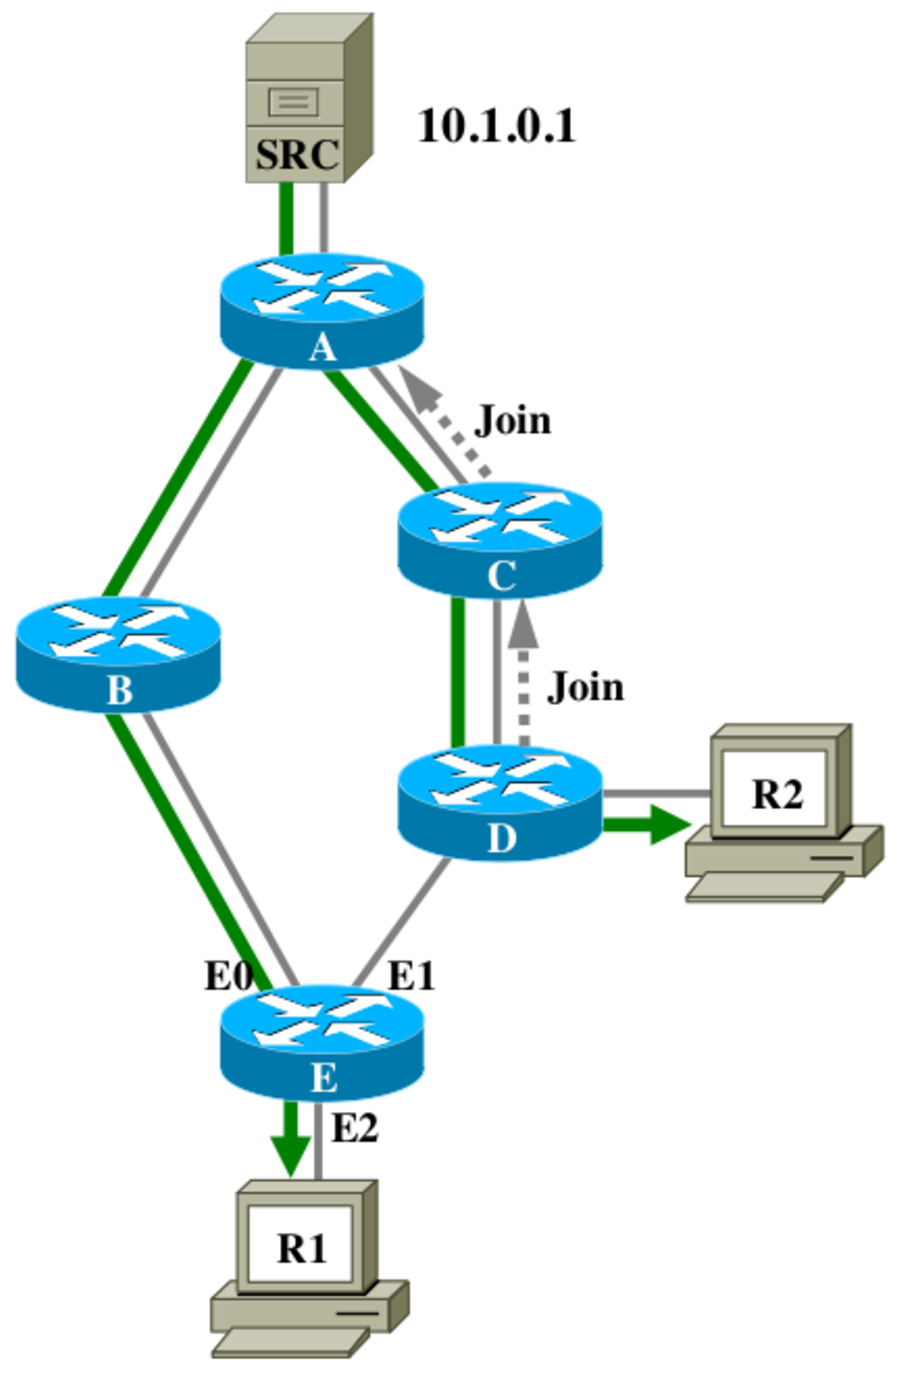
\includegraphics[width=0.3\linewidth]{images/rpf}
\caption{Reverse Path Forwarding}
\end{figure}

\section{WAN: Wide Area Networks}
Ein WAN verbindet zwei Standorte über einen Service Provider. Wichtig sind dabei folgende Punkte

\begin{enumerate}
	\item Bandbreite / Delay
	\item Sicherheit / Wer hat Zugriff auf das Netz
	\item Verfügbarkeit. Sollte mittels SLA festgehalten werden
	\item Kosten
\end{enumerate}

Im WAN Bereich wird auf den verschiedenen OSI Layern unterschiedliche Technologien eingesetzt:
\begin{itemize}
	 \item Layer 1: 
	 \begin{itemize}
	 	\item kurze Distanz: DSL
	 	\item weite Distanz: TDM, SDH
	 \end{itemize}
	\item Layer 2: 
	\begin{itemize}
		\item bis 2005: Frame Relay, ATM
		\item seit 2005: Ethernet
	\end{itemize}
	\item Layer 3: 
	\begin{itemize}
		\item seit 2000: IP-Sec / SSL-VPN
		\item seit 2002: MPLS-VPN
	\end{itemize}
\end{itemize}

\subsection{Vergleich zum LAN}
\begin{tabu} to \linewidth {|X|X|X|}
	\hline
	Bereich & LAN & WAN \\ 
	\hline \hline
	Bandbreite & 10/100/1000Mbps & 64kbps - 20Mbps\\	
	\hline
	Topologien & Extended Star Topology (Mehrer Router miteinander verbunden) & Point-to-Point, Point-to-Multipoint, Any-To-Any \\	
	\hline
	Verfügbarkeit / Redundanz & Normalerweise sehr hoch & Kosten und Nutzen: Wird meist über SLA definiert \\	
	\hline
	Verwaltbarkeit & Sehr gut, alles unter der eigenen Kontrolle & Komplett abhängig vom Service Provider \\	
	\hline
	Kosten per Mbps & 100CHF pro Gigabit Port & 50-100CHF pro Mbps im Monat \\	
	\hline
	Technologien & Ethernet & Mietleitung (Seriell), Frame Relay, DSL, ATM, SDH, MPLS \\	
	\hline
\end{tabu}

\subsection{Vergleich Overlay Modell und Peering Modell}
\begin{tabu} to \linewidth {|X|X|X|}
	\hline
	Bereich & Overlay Modell (P2P, FrameRelay) & Peering Modell (MPLS) \\ 
	\hline \hline
	Verbindungstyp & Logische End-to-End Verbindung & Any-to-Any IP Routing \\	
	\hline
	Adressierungschema & DLCI & IP Adressen \\	
	\hline
	Kosten & P2P auf L2, Kosten pro Verbindung basierend auf Bandbreite & L2 oder L3 any-to-any wobei Kosten für Zugang zum MPLS Netz basierend auf Bandbreite\\	
	\hline
	QoS & Traffic Shapping & MPLS Traffic Engineering (Header Feld) \\	
	\hline
\end{tabu}

\subsection{Serial Lines / Mietleitungen}
Serial Lines sind gemietete Leitungen welche eine synchrone Übertragung erlauben. Hierbei stellt der Provider meist ein Modem (CPE) zu Verfügung welches mit dem Router (DTE) des Kunden verbunden wird. Dies ermöglicht eine Punkt zu Punkt Verbindung zwischen zwei Standorten. Der Nachteil einer Mietleitung ist, dass sie auch gebraucht wird, wenn keinen Daten übertragen werden. Serial Lines werden mit PPP vermittelt.

\subsection{ISDN: Integrated Service Digital Network}
ISDN lösste das analoge Public Switched Telephone Network (PSTN) ab, da dieses stark limitiert war. ISDN unterstützt die Übertragung von Daten, Sprache und Video, wobei es mit einer Übertragungsrate von 64kbps für Sprachübertragung optimiert wurde. 

\subsection{DSL: Digital Subscriber Line}
DLS nutzt das bestehende Telefonkabel zur Datenübertragung. Für DSL hat man die Bandbreitenbeschränkung von 3.1kHz, wie sie im analogen Telefonanschlüssen üblich ist, aufgehoben damit die gesamte Bandbreite des Kupfers zur Verfügung steht.

\begin{description}
	\item[Symmetrical DSL] Upload und Download Geschwindigkeiten sind gleich
	\item[Asymmetrical DSL] Upload und Download Geschwindigkeiten sind unterschiedlich, wobei die Download Geschwindigkeit meist grösser ist.
	\item[Tiefpassfilter] Signalanteile mit Frequenzen unterhalb der Grenzfrequenz gehen durch, Anteile mit höheren Frequenzen werden gedämpft.
\end{description}

\subsubsection{ADSL / VDSL / VDSL2 Vectoring}
\begin{description}
	\item[ADSL: Asymmetric DSL] \hfill \\
	ADSL und ADSL2 benutzten den Frequenzbereich zwischen 138 kHz und 1,104 MHz, der in den Upstreambereich zwischen 138 kHz und 276 kHz und den Bereich für den Downstream von 276 kHz bis 1,104 MHz unterteilt ist
	\item[VDSL: Very High Speed DSL] \hfill \\
	Die VDSL-Technik wurde speziell für den Einsatz in hybriden Glasfaser-/Kupferkabelnetzen in Zugangsnetzen entwickelt. VDSL arbeitet im Frequenzbereich zwischen 138 kHz und 12 MHz mit Quadraturamplitudenmodulation (QAM). Der Frequenzbereich ist in zwei Upstream- und zwei Downstream-Bereiche unterteilt. 
	\item[VDSL 2 Vectoring] \hfill \\
	Ziel von Vectoring ist das Übersprechen in Kupferkabel zu verringern und zu kompensieren um somit höhere Datenraten zu erreichen.
\end{description}

ADSL und VSDL arbeiten auf unterschiedlichen Frequenzbereichen wobei noch zwischen Up und Downstream unterschieden wird. VSDL bietet im Gegensatz zu ADSL zwar einen höheren Durchsatz, ist dafür in seiner Reichweite begrenzt.

\begin{figure}[h]
	\centering
	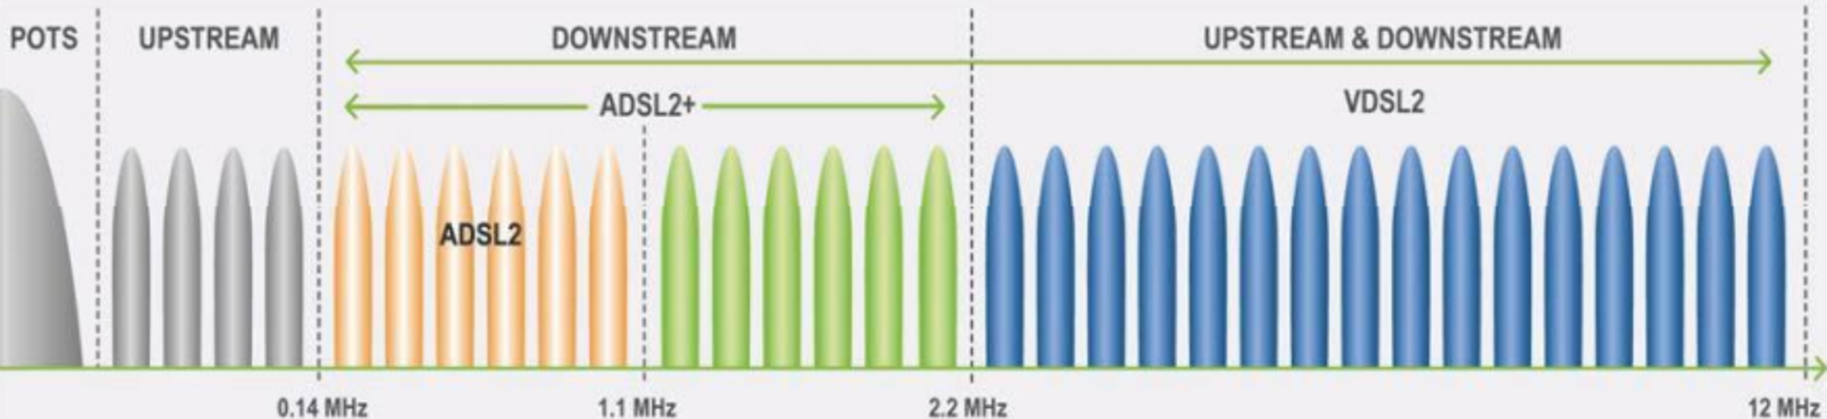
\includegraphics[width=0.7\linewidth]{images/pots_adsl_vdsl}
	\caption{Frequenzen POTS/ADSL/VDSL}
\end{figure}

\subsubsection{SDH: Synchronous Digital Hierarchy}
SDH  moduliert die Daten in Envelopes bestehend aus Reihen und Spalten. Ein SDH Netzwerk ist meistens ringförmig aufgebaut. Es gibt zwischen zwei Nodes in jede Richtung jeweils 2 Fibers (ergo Total 4). Pro Richtung wir jedoch nur eine verwendet. Die zweite Fiber dient einzig der Aufallsicherheit.
git 
\subsection{DOCSIS: Data over Cable Service Interface Specification}
DOCSIS ist ein Standard für die Datenübertragung mit Kabelmodems im TV-Kabelnetz, wie es in der Schweiz die Cablecom nutzt. Für Europa existiert ein abgeänderter Standard (EuroDOCSIS) mit einer Bandbreite von 8 MHz im Downstream-Kanal, gegenüber 6 MHz im amerikanischen DOCSIS. Seit DOCSIS 3.0 sind Dantenraten von 100MBit/s möglich. Der Nachteil dieser Technologie ist, dass auf die Bandbreite auf der letzten Meile geshared ist.

\subsection{FTTH: Fiber to the Home}
Bei FTTH wird anstatt Kupfer optische Glasfaserkabel für die Datenübertragung verwendet. Es existieren zwei FTTH Varianten:

\subsubsection{Layer 1}
Bei dieser einfacheren, jedoch teureren Variante bekommt jeder Haushalt/Organisation ein eigenes Glasfaserkabel in das Gebäude gezogen. 

\subsubsection{Layer 2}
Hierbei wird eine Haushalt/Organisation an einen Switch in der Verteilzentrale angeschlossen und die Dienste des Service Providers über VLANs getrennt. Ein Provider benötigt maximal 3 VLAN (Data, Video, Voice)
	
\subsection{PPP: Point to Point Protocol}
PPP hat die Aufgabe, Punkt-zu-Punkt-Verbindungen zu initialisieren, aufrecht zu erhalten und auch wieder zu beenden. PPP ist für die Authentifizierung, die Aushandlung der Paketgröße, die Vergabe von IP-Adressen und die Verschlüsselung der Daten zuständig. PPP arbeitet auf Layer 2. PPP überträgt verschiedenste L3 Protokolle und ist von diesen unabhängig. Typische Punkt-zu-Punkt-Verbindungen sind Verbindungen in leitungsvermittelnde Netze:
\begin{itemize}
	\item Wählverbindungen über das analoge Telefonnetz (mit analog-Modem)
	\item Wählverbindungen über GSM (Mobilfunk)
	\item Wähl- oder Festverbindungen über ISDN
	\item serielle Verbindungen
	\item ATM-Verbindungen (PPP over Ethernet bei DSL)
\end{itemize}

\paragraph{LCP: Link Control Protocol}
PPP nutzt LCP zum Aufbau, Konfiguration und Testen einer Datenverbindung

\begin{figure}[h]
	\centering
	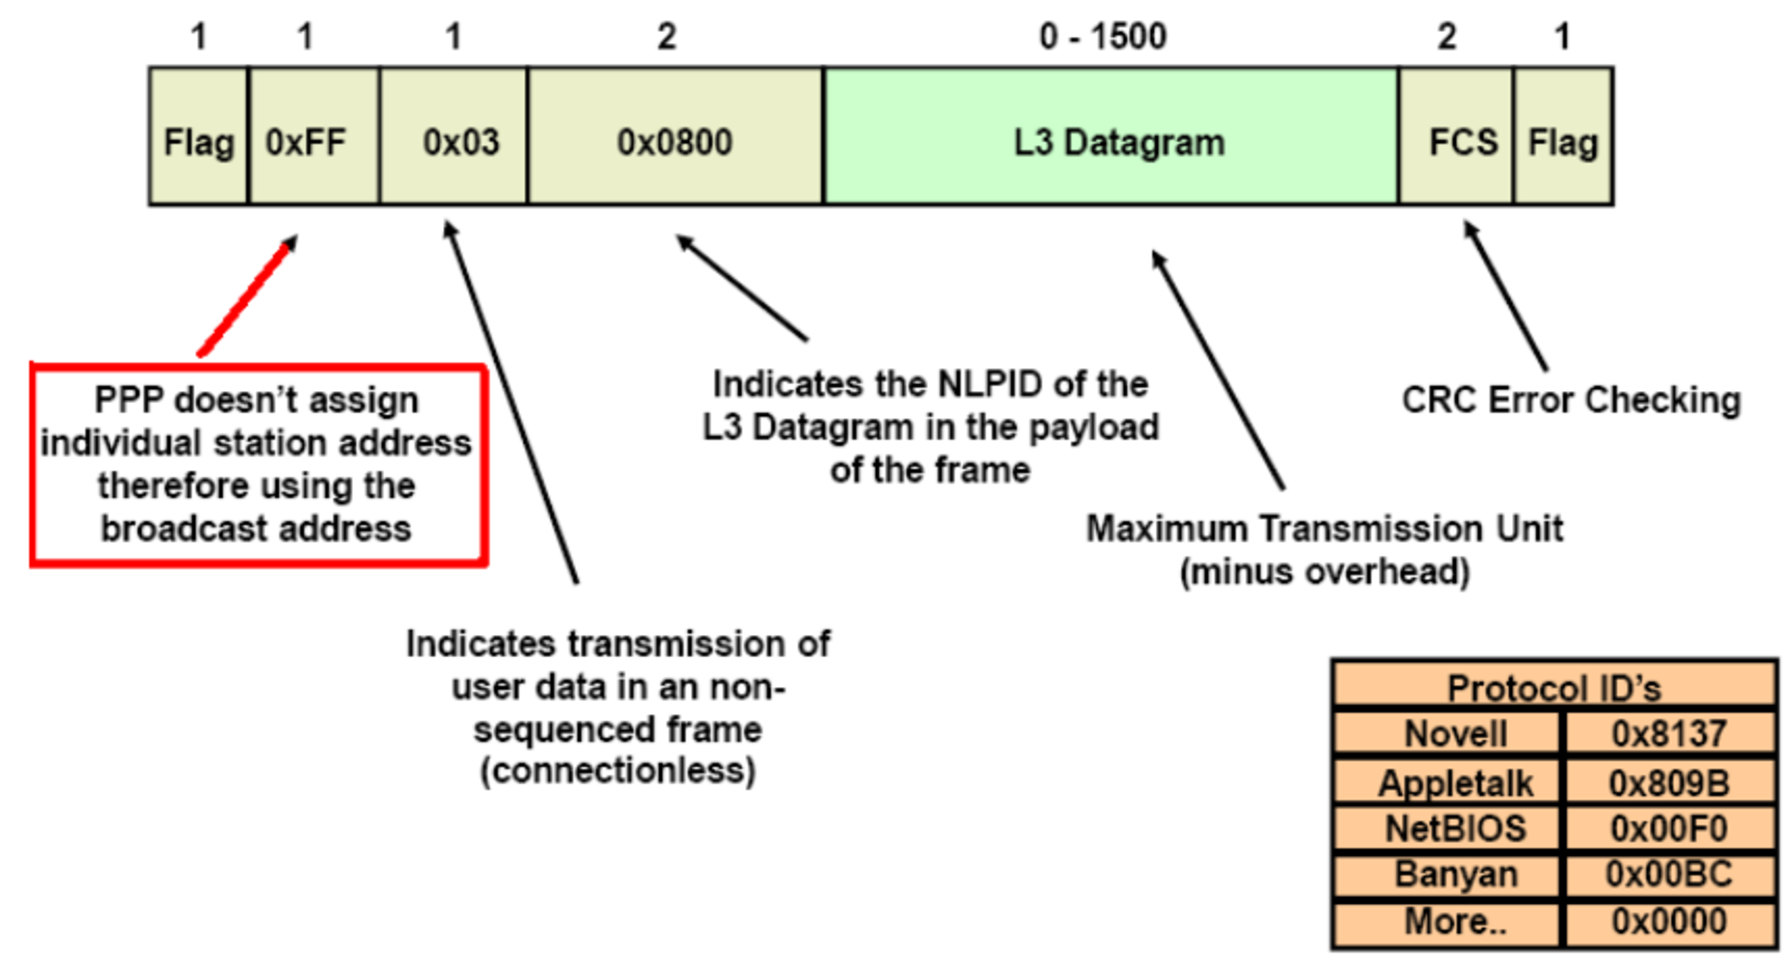
\includegraphics[width=0.7\linewidth]{images/ppp_frame}
	\caption{PPP Frame}
\end{figure}


\subsubsection{PAP: Password Authentication Protocol}
PAP ist ein Protokoll für die Authentifizierung über PPP mittels Benutzername und Passwort. Die Daten werden unter PAP unverschlüsselt übertragen. Ebenfalls gibt es kein Maximum bei den Authentifizierungsversuchen, womit Brutforce Attacken möglich sind.

\subsubsection{CHAP: Challenge Handshake Authentication Protocol}
CHAP ist wie PAP ein Protokoll für die Authentifizierung über PPP, wobei die Sicherheitslücken von PAP zu verringern.
\begin{enumerate}
	\item Hat sich der Client eingewählt wird er vom Server zur Authentifizierung aufgefordert. Der Server schickt dazu eine zufällige Zahl (Challenge) an den Client.
	\item Der Client bildet aus der Zufallszahl und dem Passwort einen Hashwert (z. B. mit MD5) und überträgt ihn an den Server (Response).
	\item Der Server bildet ebenfalls aus der Zufallszahl und dem hinterlegten Passwort einen Hashwert. Stimmt der Hashwert des Clients mit dem des Servers überein wird die Authentifizierung akzeptiert (Accept). Wenn nicht, wird sie abgelehnt (Reject).
\end{enumerate}

\subsubsection{PPPoE: Point to Point Protocol over Ethernet}
PPPoE ist ein Netzwerkprotokoll, dass PPP Frames in Ethernet Frames verpackt. Es wird für ADSL/VDSL und FTTH verwendet.

\subsection{RADIUS: Remote Authentication Dial-In User Service}
Radius ist ein Client-Server-basiertes Sicherheitsprotokoll zur Authentifizierung, Authorisierung und zum Accounting (AAA) von Benutzern in einem Netzwerk. Radius arbeitet mit dem Challenge-Response-Verfahren und unterstützt die zentrale Administration von Benutzerdaten. RADIUS arbeitet mit UDP. Möchte ein Client sich im Netzwerk authentifizieren, sendet er einen Request an den RADIUS Server mit Benutzernamen und Passwort. Der RADIUS Server überprüft und Daten und gibt ein Accept (Ip-Adresse und weitere Konfigurationparameter) oder Reject zurück.

\subsection{Framerelay}
Im Gegensatz zu Ethernet, welches die Daten an alle Teilnehmer Broadcasted erstellt Framerelay eine virtualisierte Punkt zu Punkt Verbindung. Das heisst Frame Realy ist im Vergleich zu Ethernet verbindungsorientiert. FR ist der Versuch Ethernet im WAN zu simulieren. Framerelay arbeitet auf L2 und ist Paket geswitched. Framerelay unterstützt im Gegensatz zu Ethernet QoS. Man unterscheidet zwischen zwei Verbindungstypen:

\begin{description}
	\item[PVC: Permanent Virtual Circuits] Permanente Verbindung bei welcher kein Verbindungsaufbau nötig ist. Dies wird insbesondere in kleineren Netzwerken benutzt
	\item[SVC: Switched Virtual Circuits] Temporäre Verbindung mit Sessions. Hierbei wird nur bei Bedarf die Leitung genutzt. Sie hat einen Verbindungsaufbau, Transfer und Abbauphase. Dies findet insbesondere in grossen Netzwerken anwendung.
\end{description}

\paragraph{DLCI: Data Link Connection Identifier}
\begin{itemize}
	\item Pro physichen Link kann es mehrere virtuelle Links geben
	\item Ein DLCI ist die Adresse des virtuellen Interfaces innerhalb des physischen Kabel. Es kann maximal 1024 DLCI pro physisches Kabel geben, da im FrameRelay Header 10Bits für DLCI Informationen vorhanden sind.
	\item DLCI's haben lokale Signifikanz (zwischen zwei L2 Switches)
	\item Ist auf einem Switch Port bereits ein DLCI eingetragen, wird für die neue Verbindung einfach die nächst höhere genommen.
\end{itemize}

\subsubsection{Traffic Control (QoS)}
Frame Relay hat im Gegensatz zu Mietleitungen eine grössere physikalische Bandbreite. Bei der Mietleitung muss zu viel Traffic gepuffert und zeitversetzt versendet werden. Bei FrameRelay hat es beim Eingang einen sogenannten Shaper. Dieser prüft dass der Kunde sich an die abgemachten Geschwindigkeiten gemäss dem Vertrag (SLA) hält. Falls die Bandbreite überschritten wird, werden die übrigen Daten gepuffert.
\begin{description}
	\item[CIR: Commited Information Rate] \hfill \\
	Ist die garantierte Bandbreite innerhalb eines Virtual Circuit unter normalen Bedingungen. Wird diese Schranke übertreten, wird die Pakete mit dem DE Bit (Discard Eligibility) markiert.
	\item[EIR: Extended Information Rate] \hfill \\
	Wird diese Schranke übertreten, werden die Pakete gedropt.
	\item[AR: Access Rate] \hfill \\
	Die effektive physische Bandbreite
	\item[BECN: Backward Explicit Congestion] \hfill \\ Ist eine Meldung in Richtung Sender, dass ein Frame Relay Knoten überlastet ist. Der Shaper reduziert daraufhin den Traffic. BECN ist Teil von QoS
	\item[FECN: Forward Explicit Congestion Notification]\hfill \\ Ist eine Meldung in Richtung Empfänger, dass ein Frame Relay Knoten überlastet ist. Der Shaper reduziert daraufhin den Traffic. FECN ist Teil von QoS
\end{description}

\subsection{ATM: Asynchronous Transfer Mode}
\begin{itemize}
	\item ATM arbeitet mit Zellen in der Grösse von 53 Bytes
	\item Wurde für UMTS, ADSL genutzt
	\item Skalliert schlechter wie MPLS
	\item Cell-Switching kann aufgrund der fixen Zellgrösse in Hardware umgesetzt werden. Dies ist brachte früher einen grossen Geschwindigkeitsgewinn. Aktuelle Ethernet Software Switches erreichen aber heutzutage gleiche Geschwindigkeiten.
	\item VPI: Virtual Path Identifier = Identifiziert einen Pfad innerhalb eines ATM Netzwerkes zwischen zwei Knoten und hat wie die DLCI nur lokal signifikanz.
	\item VCI: Virtual Channel Identifier = Wird für das Multiplexing benögt und erlaub das Unterscheiden mehrere Datenströme. Ist eine Zahl die hochgezählt wird, sobald bereits eine Verbindung besteht.
	\item VCC: Virtual Channel Connection =  Ein VCC ist eine einzelne Verbindung zwischen zwei ATM Endsystemem. 
	\item VPC: Virtual Path Connection = Bündeln mehrere VCI in einem physischen Medium
\end{itemize}

\subsection{MPLS: Multiprotocol Label Switching}
\begin{itemize}
	\item Nutzt das Beste aus Layer 2 (effizient, Traffic Engineering über FEC (Forwarding Equivalence Class)) und Layer 3 (Flexibel, skalierbar) und wird deshalb auch Layer 2.5 Protokoll genannt
	\item Leitet Pakete aufgrund von Labels weiter (Label Switching). IP Adressen werden innerhalb eines MPLS Netzwerkes nicht nötig
	\item Wie bei die DLCI bei Frame Relay sind die Labels nur lokal signifikant. Sie können also während dem Transport zwischen Router und Router wechseln.
	\item MPLS wird von ISP angeboten
	\item MPLS nutzt BGP um die verschiedenen Router zu synchronisieren
\end{itemize}
	
\subsubsection{MPLS Router}
\begin{description}
	\item[LSR: Label Switch Router] \hfill \\ LSR = Router innerhalb der MPLS Wolke. Wird vom Provider betrieben.
	\item[P: Provider Router] \hfill \\
	Switched Pakete mit Labels im MPLS Netzwerk und ändern allenfalls die Labels (Label Swap)
	\item[PE: Provider Edge Router] \hfill \\
 Setzt (Label push) und entfernt (Label pop) die Labels
	\item[CE: Customer Edge Router] \hfill \\
	Verbindet das Kundennetzwerk mit dem MPLS Netzwerk
	\item[Route Target] \hfill \\
	Pro Kunde ein eindeutiger Identifier
	\item[Route Distinguisher] \hfill \\ 
	Pro VPN Route wird ein eindeutiger Identifier gesetzt. Normalerweise wird die AS Nummer genommen.
	\item[VRF: Virtual Routing and Forwarding] \hfill \\ Erlaubt mehrere Routing Tabellen auf einem physischen Router. Dies erlaubt überlappende IP-Netze (Overlapping Networks). Das VRF ist das Label für ein VPN. Zusätzlich kommt auf L3 ein IGP Label hinzu (lokal signifikant)	
\end{description}

\begin{figure}[h]
	\centering
	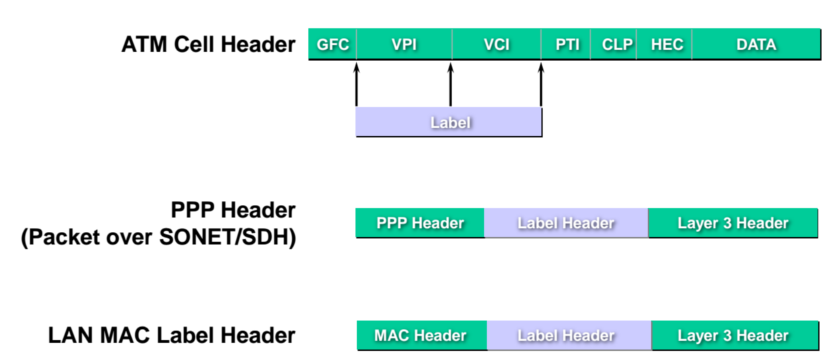
\includegraphics[width=0.7\linewidth]{images/mpls_label.png}
	\caption{MPLS Label für L2 Protokolle}
\end{figure}

\subsubsection{Ablauf}
Bei der Kommunikation von einer Niederlassung zur einer zweiten über MPLS werden folgende Stationen durchschritten:
\begin{enumerate}
	\item CE Router der ersten Nierlassung leitet den Verkehr an PE Router weiter
	\item Der PE Router fügt ein VPN Label hinzu (falls MPLS VPN verwendet wird). Ebenfalls wird anhand der IP-Zieladresse des Pakets ein Destination Label angehängt. Danach leitet der PE das Paket dem LSR weiter.
	\item Der LSR leitet die Pakete anhand seiner Destination Labels weiter. Sie ändern diese höchstens, da die Labels nur lokal signifikant sind.
	\item Beim zweiten PE Router angekommen, wird das Destination Label entfernt und gemäss Destination IP zum CPE geroutet. 
\end{enumerate}	


\subsubsection{LDP: Label Distribution Protocol}
Ist verantwortlich über den Austausch der Labels. Es gibt zwei Varianten der Verteilung: 
\begin{enumerate}
	\item Control Driven: Die Labelinformationen werden von Routern bekannt gegeben. Dieses Methode ist schnell, verursacht jedoch Overhead, da sämtliche Routen verteilt werden.
	\item Data Driven: Der Pfad wird erst dann aufgelöst wenn wirklich ein Paket mit Label anliegt.
\end{enumerate}
Ein LDP Rooter findet seine Nachbarn mittels dem HELLO Protokoll. Er versendet dabei periodisch UDP Multicast Nachrichten um neue Nachbarn zu erkennen.

\paragraph{Label Distribution Vorgang}
\begin{enumerate}
	\item Traditionelle IP Routing Protokolle bilden Routing Tables
	\item Jeder LSR (Label Switch Router) weist  unabhängig von anderen LSR's allen Destinations in seiner Routing Tabelle ein Out-Label zu. 
	\item LSR's geben die zugewiesenen Label Informationen an andere LSR mittels LDP weiter. 
	\item jeder LSR bildet seine Label Information Base (LIB) anhand der erhaltenen Informationen. Ein Eintrag in der LIB wird FEC (Forwarding Equivalence Class) genannt.
\end{enumerate}
\begin{figure}[h]
	\centering
	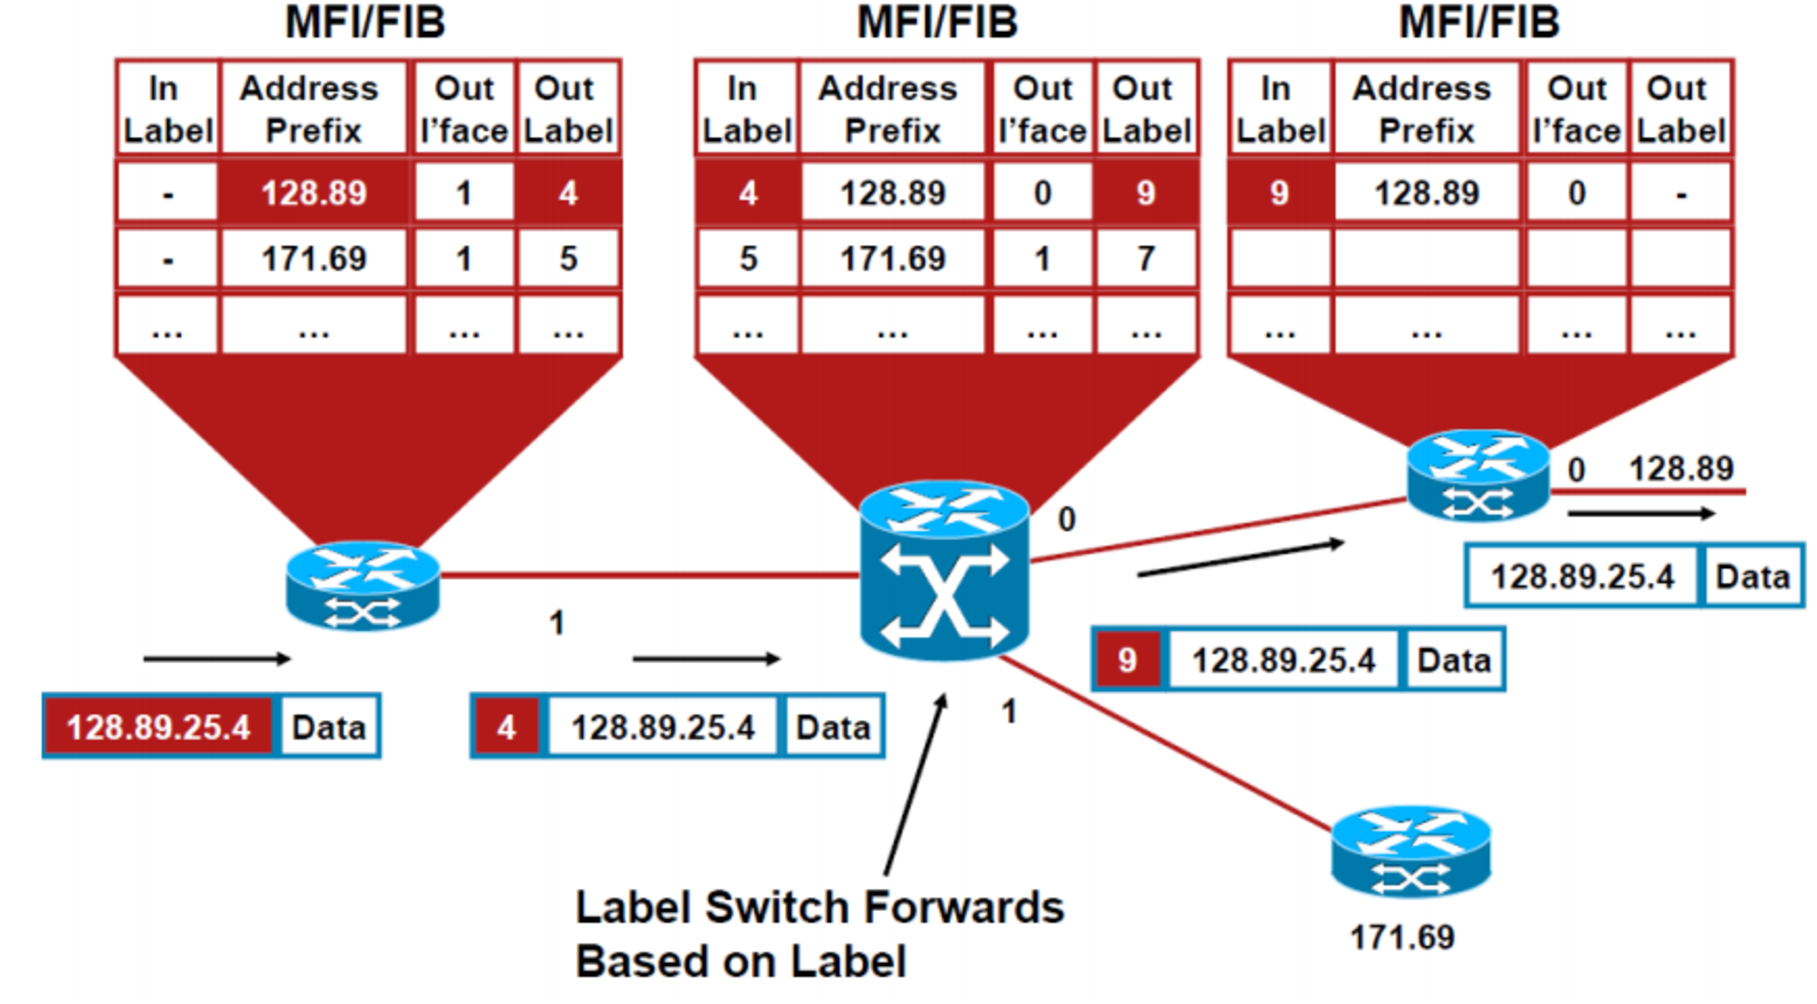
\includegraphics[width=0.7\linewidth]{images/mpls_ldp.pdf}
	\caption{MPLS Label für L2 Protokolle}
\end{figure}

\paragraph{Label Stacking}
Es ist möglich mehrere Labels einem Paket anzuhängen um so mehrere MPLS Verbindungen in einander zu verschachteln. 

\subsection{MPLS VPN}
\begin{itemize}
	\item Im Gegensatz zum klassischen VPN (nur L3) geht eine MPLS Verbindung nicht über das Internet sondern nur über einen einzigen ISP.
	\item Unterstützt QoS (Quality of Service)
	\item Ein VPN wird eindeutig mittels Label und VPN-ID identifiziert (VRF)
\end{itemize}

\subsubsection{Layer 2 VPN}
Es gibt drei Typen von L2 VPN. Alle benutzen Pseudo Wires mit VC Labels.
\begin{enumerate}
	\item VPWS: Virtual Private Wire Service (Point to Point)
	\begin{enumerate}
		\item Layer 2 Tunneling Protocol (L2TP): L2 VPN über IP (Internet)
		\item Any Transport over MPLS (AToM): L2 VPN über MPLS
	\end{enumerate}
	\item VPLS: Virtual Private LAN Service (Point to Multipoint)
	\begin{enumerate}
		\item Benötigt MPLS
		\item Nutzt Split Horizon um Loops zu unterbinden
	\end{enumerate}
\end{enumerate}

\subsection{MPLS QoS}
\begin{itemize}
	\item QoS wird auf Layer 3 in dem Feld DSCP definiert
	\item Will man QoS auf MPLS machen, muss das DSCP Feld von IP auf das EXP Feld von MPLS gemapt werden.
	\item Bei Routing Protokollen besteht das Problem, dass immer der beste Pfad genommen wird. Um trotzdem QoS einzusetzen wird als next Hop ein Tunnel angegeben. 
\end{itemize}

\subsection{Multiplexing}
\begin{description}
	\item[SDM: Space Division Multiplex] \hfill \\
	Übertragung von mehreren Signalen über mehrere Übertragungswege
	\item[FDM: Frequency Division Multiplex] \hfill \\
	Gleichzeitiges Übertragen auf unterschiedlichen Frequenzen innerhalb eines Frequenzbandes
	\item[TDM: Time Division Multiplex] \hfill \\
	Die komplette Bandbreite steht einem Kanal für ein bestimmtes Zeitfenster zur Verfügung.
	\item[WDM: Wavelenght Division Multiplex] \hfill \\
	Ist ähnlich wie FDM, wobei das Signal einer speziellen Lichtwellenlänge zugeordnet wird.
	\item[OFDM: Orthogonal Frequency Division Multiplex] \hfill \\
	Bandbreitegewinn durch überlappen der Signale. Jedes Nachbar Signal startet exakt in der Mitte des vorherigen Signals
	\item[CDM: Code Division Multiplex] \hfill \\
	Die Signale werden mit einer unterschiedlichen Codierung übertragen.
\end{description}

	
\section{IPv6}
IPv6 ist die Antwort auf die grosse Adressknappheit die unter IPv4 existiert und mittels NAT gelindert aber nicht gelöst wurde. Aktuell sind ca. 10-15\% des gesamten Internetverkehrs IPv6. 

\subsection{IPv4 Transition }
\begin{description}
	\item[Dualstack] Hierbei hat ein Client zwei Protokoll Stacks. Einerseits einen IPv4-, und anderseits einen IPv6-Stack. Es wird anhand der der Destination Address entschieden, welcher Stack verwendet wird. Falls beide Protokolle verfügbar sind, wird IPv6 bevorzugt. Der Fallback auf IPv4 bis zu 30 Sekunden dauern kann, wurde der Happy Eyeballs Algorithmus entwickelt. Dieser erlaubt das öffnen von zwei parallel laufenden Verbindungen (1x IPv4 und 1x IPv6). Der Fallback kann somit verkürtzt werden, falls die Webseite kein IPv6 anbietet.
	\item[6in4 (Overlay Tunnels)] Hierbei wird IPv6 in IPv4 Datgrams gekapselt. (20Byte IPv4 Header, MTU $\Rightarrow$ Fragmentation)
	\item[GRE: Genereic Routing Encapsulation] Hiermit lassen sich IP-Protokolle tunneln und somit IPv6 Verbindungen über ein IPv4 Netzwerk umsetzen.
	\item[6to4] \hfill \\
	Hierbei wird die IPv4 Adresse hexadezimal in eine IPv6 ''codiert''. 6to4 hat immer den IPv6 Prefix von 2002::/16. IPv4 a.b.c.d = IPv6 2002:0a0b:0c0d::
	\item[6RD: IPv6 Rapid Deployment] \hfill \\
	6RD verfolgt die gleiche Idee wie 6to4 mit dem Unterschied, dass sie keinen speziellen Adressbereich (2002::/16), sondern den IPv6 Adressbereich des Providers verwendet. Die 6RD Domain wird so berechnet, dass man den gegebenen ISP 6RD-Prefix verwendet und diesen mit der IPv4 des CE (umgerechnet in Hex) auf /64 erweitert. Ist der Provider Range nicht genau 32 Bits lang, werden die Bits der IPv4 Adresse von rechts nach links genommen.
	\begin{figure}[h]
		\centering
		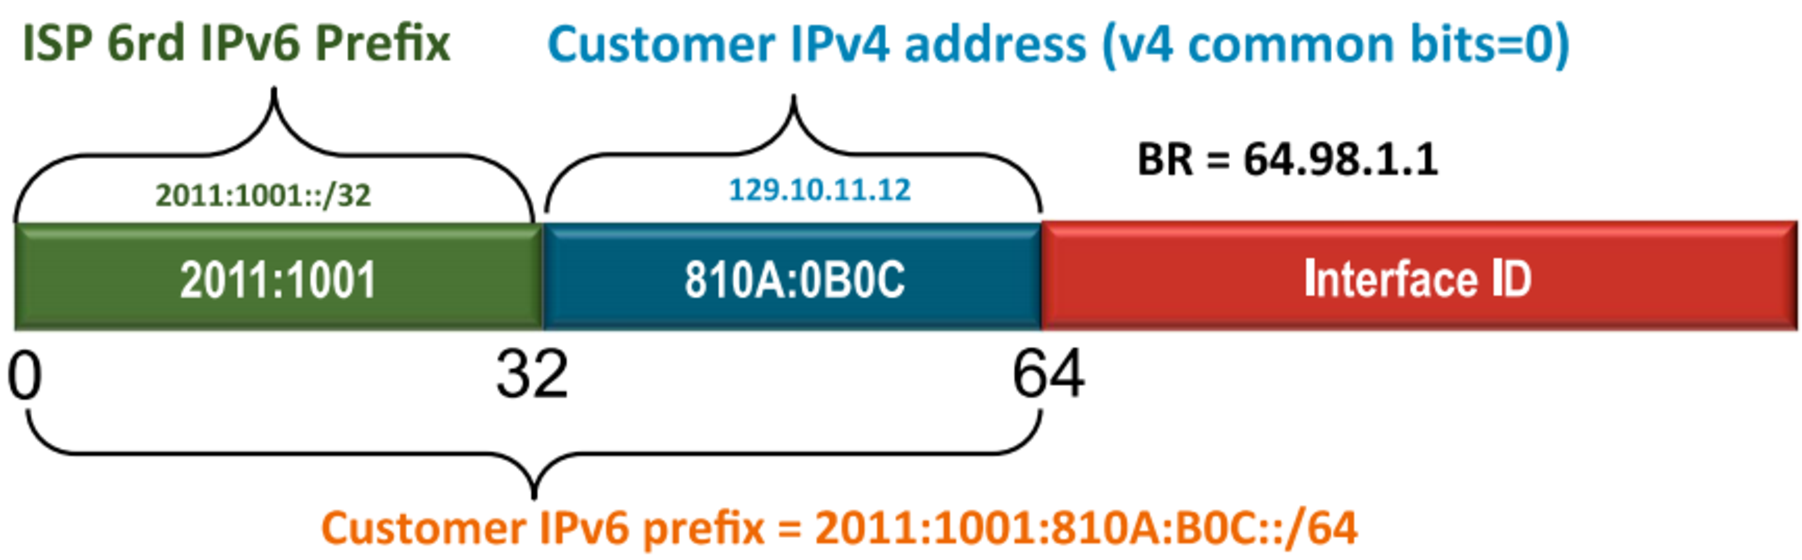
\includegraphics[width=0.4\linewidth]{images/6rd_address_prefix}
		\caption{6RD Prefix Calculation}
	\end{figure}
	
	\begin{figure}[h]
		\centering
		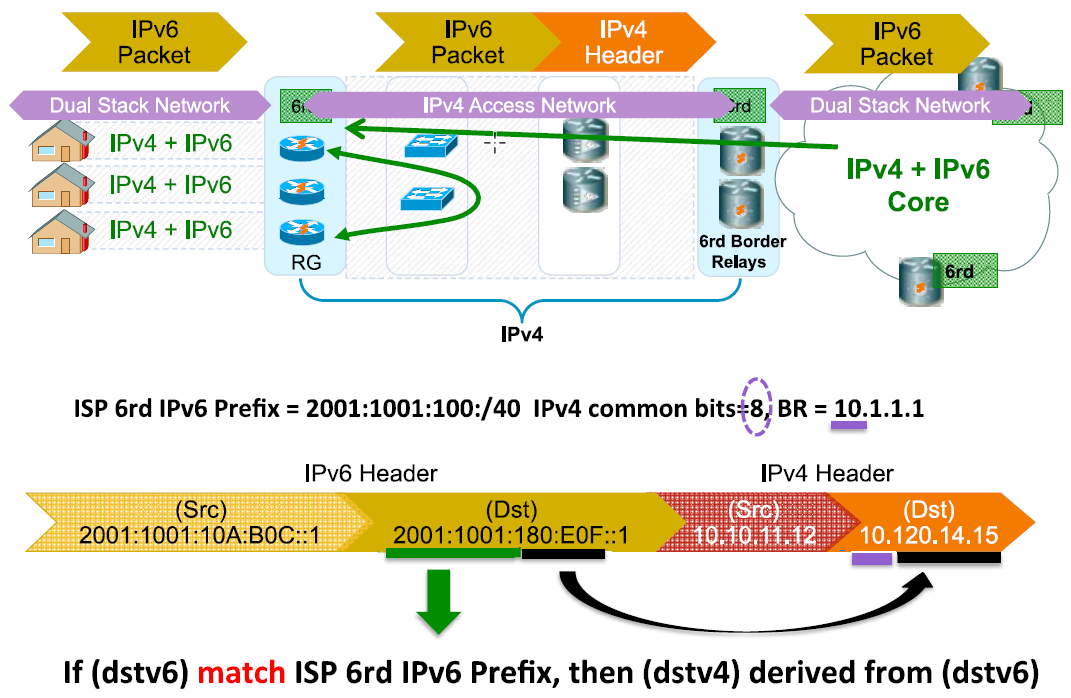
\includegraphics[width=0.4\linewidth]{images/6rd_transmission}
		\caption{6RD Prefix Calculation}
	\end{figure}

\end{description}

\subsection{IPv6 Header}
Der IPv6 Header wurde vereinfacht.
\begin{itemize}
	\item Header length wurde weggelassen, da diese neu fix 40Bytes gross ist
	\item Die Payload Length definiert die Länge des Payloads inklusive den Extension Headers. Der IPv6 Payload $2^{16} = 65536$Bytes gross sein
	\item Es wurden nur noch die essentiellen Headers eingefügt. Selten genutze Header können in speziell dafür vorgesehen Extension Headers vor den Payload gepackt werden. Mehrerere Extension Headers werden über das Next Header Feld verlinkt.
	\item Fragment Offset wurde weggelassen, da es unter IPv6 keine Fragmentierung mehr gemacht wird. Falls dies trotzdem erwünscht ist, muss es über die Extensions Headers gelöst werden.
	\item Header Checksum wurde weggelassen, da Fehler auf L3 sehr unwahrscheinlich sind. Dies erlaubt schnellers Routing, da die Checksumme nicht für jedes Paket berechnet werden muss. Fehlerbehandlung wird unter IPv6 nur noch auf L2 und L4(UDP/TCP) gemacht.
	\item Type of Service (QoS) wurde durch das 8Bit grosse Traffic Class ersetzt. Zusätzlich kann über das 20Bit grosse Flow Label, QoS Parameter übergeben werden.
	\item IPv6 unterstützt Extensions Headers die dem Basis Header angehängt werden.
	\item Das Protokoll Feld wurde durch das Next Header Feld ersetzt. Es definiert welches Protokoll auf dem nächst höheren Layer verwendet wird (TCP/UDP). Falls Extension Headers verwendet werden, wird darüber der Verweis auf den nächsten erweiternden Header gemacht.	
	\item Es gibt keine Fragmentierung mehr. Ist die MTU zu gross für einen Link, returniert dieser eine Fehlermeldung (Too Big) dass der Client Pakete mit kleinerer MTU sendet. (MTU Discovery)
\end{itemize}
\begin{figure}[h]
	\centering
	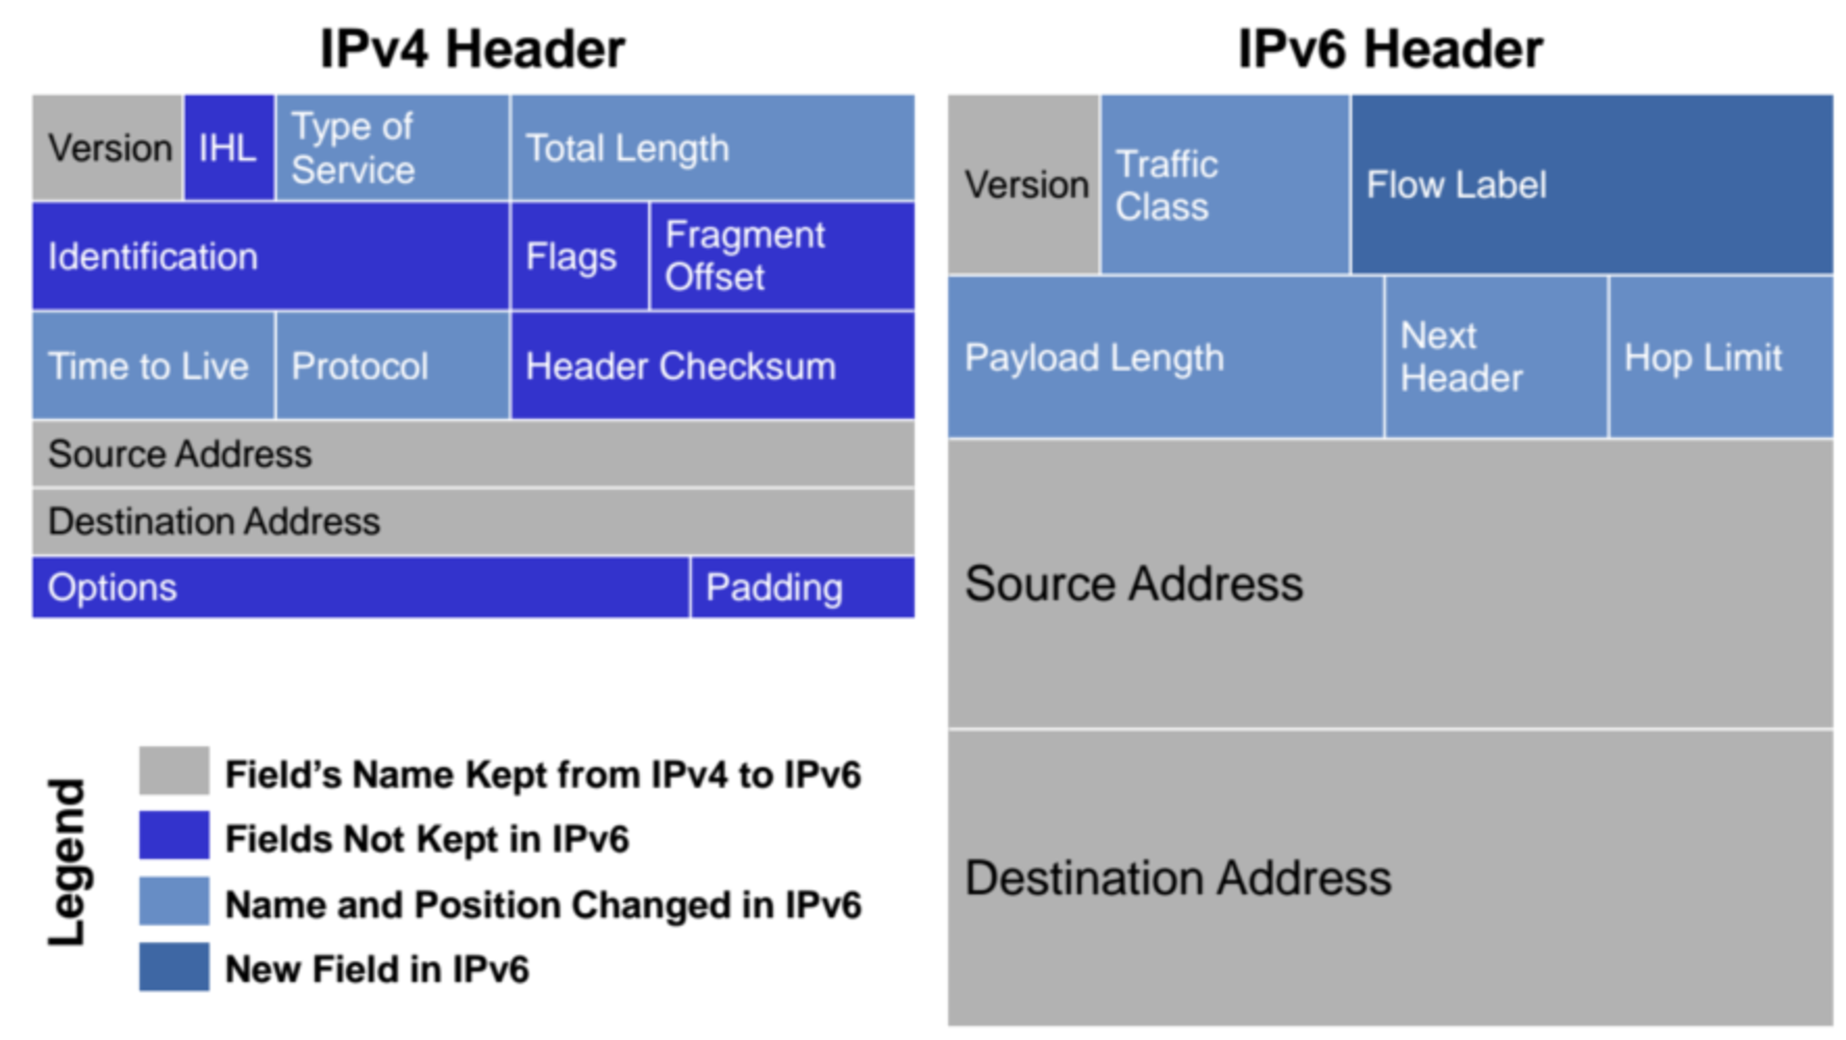
\includegraphics[width=0.5\linewidth]{images/ipv6_headers.pdf}
	\caption{IP Header im Vergleich}
\end{figure}

\begin{figure}[h]
	\centering
	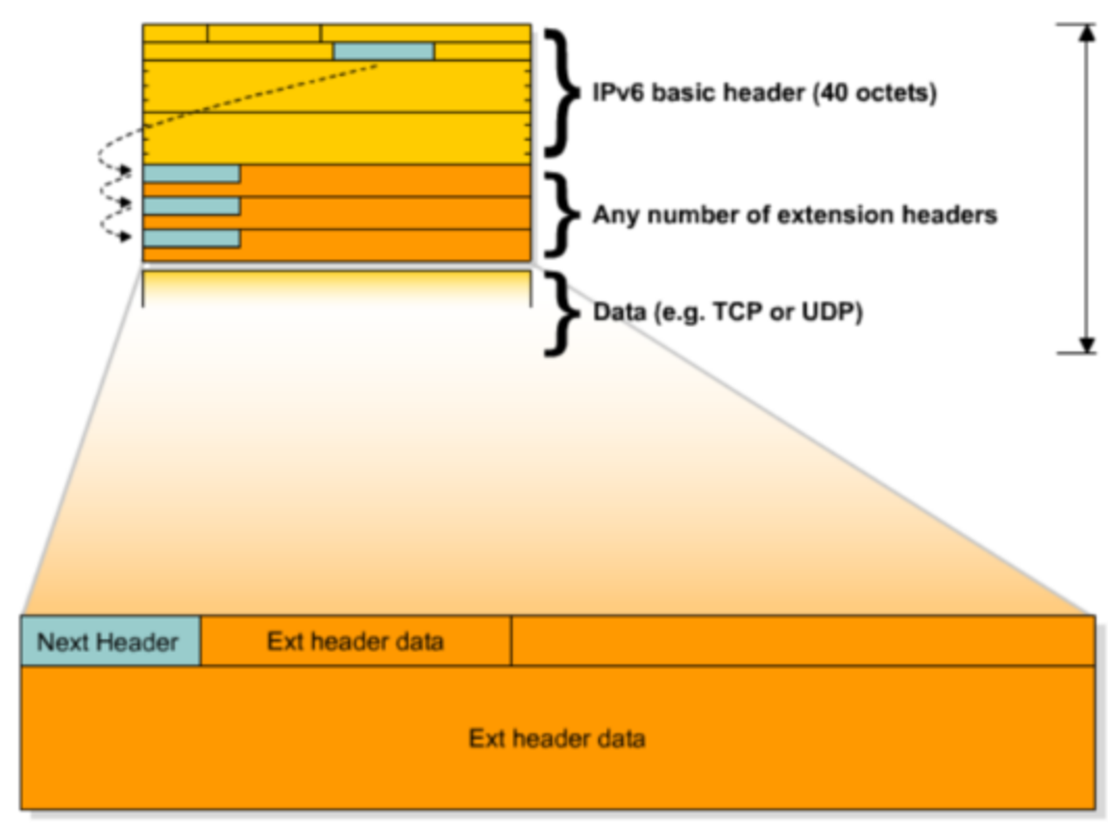
\includegraphics[width=0.5\linewidth]{images/extension_header.pdf}
	\caption{Extension Headers}
\end{figure}

\subsection{Adressierung}
\begin{itemize}
	\item 128Bit lange hexadezimale Adresse (8x16Bit = 8xQuad Nibbles)
	\item $3.4 \cdot 10^{38}$ mögliche Adressen
	\item Leading Zero können weggelassen werden
	\item Ganze 0-Blöcke können mit einem '::' ersetzt werden. Pro IPv6 Adresse ist nur ein '::' erlaubt, da ansonsten nicht mehr unterschieden werden kann, wo wievielte 0-Blöcke eingesetzt werden müssen.
	\item Die Loopback Adresse lautet ::1 (= 127.0.0.1)
	\item Die default Route lautet ::/0 und wird auch als platzhalter verwendet, wenn keine andere Adresse verfügbar ist. 
	\item Normalerweise ist eine IPv6 Adresse wie folgt aufgebaut: Das pendant zur öffentlichen IPv4 Adresse wird Global Unicast Address genannt.
	\begin{itemize}
		\item 48 Bit Provider
		\item 16 Bit Site
		\item 64 Bit Host
		\item und startet mit 2001::/16 (IANA allocated space)
	\end{itemize}
	\item Unterstützt auch Anycast Adressen. (one-to-one-of-many / one-to-nearest) Bei Anycast haben mehrere Clients die selbe IPv6 Adresse. Der Sender sendet die Pakete immer an den nächsten Knoten.
\end{itemize}

\subsection{Adress Scopes}
IPv6 Adressen werden in drei Scopes unterteilt:
\begin{description}
	\item[Link Local] \hfill \\ 
	FE80::/10 sind Link Local Adressen und werden nicht geroutet. Eine Link Local Adresse ist das pendant für die MAC-Adresse, jedoch auf L3. Diese gilt nur für  ein Interface.
	\item[Unique Local] \hfill \\
	FC00::/7 sind Unique Local Adressen, welche nur im lokalen Netz verwendet werden. Sie können nicht geroutet werden.
	\item[Global] \hfill \\
	Global Unicast Adresses sind das pendant zur öffentlichen IPv4 Adresse
\end{description}

\subsection{SLAAC: Stateless Address Autoconfiguration}
Dient der automatischen Konfiguration von IPv6 Adressen. Ein Host erzeugt sich unter Zuhilfenahme zusätzlicher Informationen sein IPv6 Konfiguration für sein Interface selbständig. Um SLAAC verwenden zu können ist eine Subnetzmaske von /64 nötig. Da SLAAC keine Möglichkeit vorsieht um den DNS Server zu konfigurieren ist diese Variante in der Praxis eher irrelevant.

\begin{enumerate}
	\item Zuerst wird die Link Local Adresse berechnet (EUI-64): 
	\begin{enumerate}
		\item 7Bit im ersten MAC-Block (U Bit) auf 1 setzen (IEEE administrated). 
		\item 8Bit im ersten MAC-Block (G Bit) auf 0 setzen (Unicast Adress)
		\item In der Mitte der MAC Adresse das FF:FE einschieben
		\item Den Link Local Prefix FE80::/10 voranstellen
	\end{enumerate}
	\item Link Local Adresse wird mittels Neighbor Discovery auf seine Eindeutigkeit geprüft. Ist sie eindeutig wird sie dem Interface hinzugefügt
	\item Der Client sendet eine Router Solicitation 
	\item Bekommt er vom Router eine Antwort (Router Advertisement) verwendet er den Netzteil der Router Source Adresse (/64) als seinen Prefix.
	\item Zusätzlich wird die komplette Source Adresse des Router als default Gateway verwendet
\end{enumerate}

\subsubsection{EUI-64: Extended Unique Identifier}
Hierbei wird die 48Bit lange MAC Adresse genommen und auf 64Bits erweitert, damit sie als eindeutige IPv6 Adresse verwendet werden kann. Dazu wird in der Mitte der MAC Adresse ein "FF:FE" eingeschoben. (falls keine Privacy Extension) Zusätzlich wird das 2Bit von rechts im ersten Block (Individual/Group Bit der MAC Adresse) geflipt. Dies erlaubt einer Station sich eine eindeutige IPv6 Adresse zuzuweisen. 
\begin{figure}[h]
	\centering
	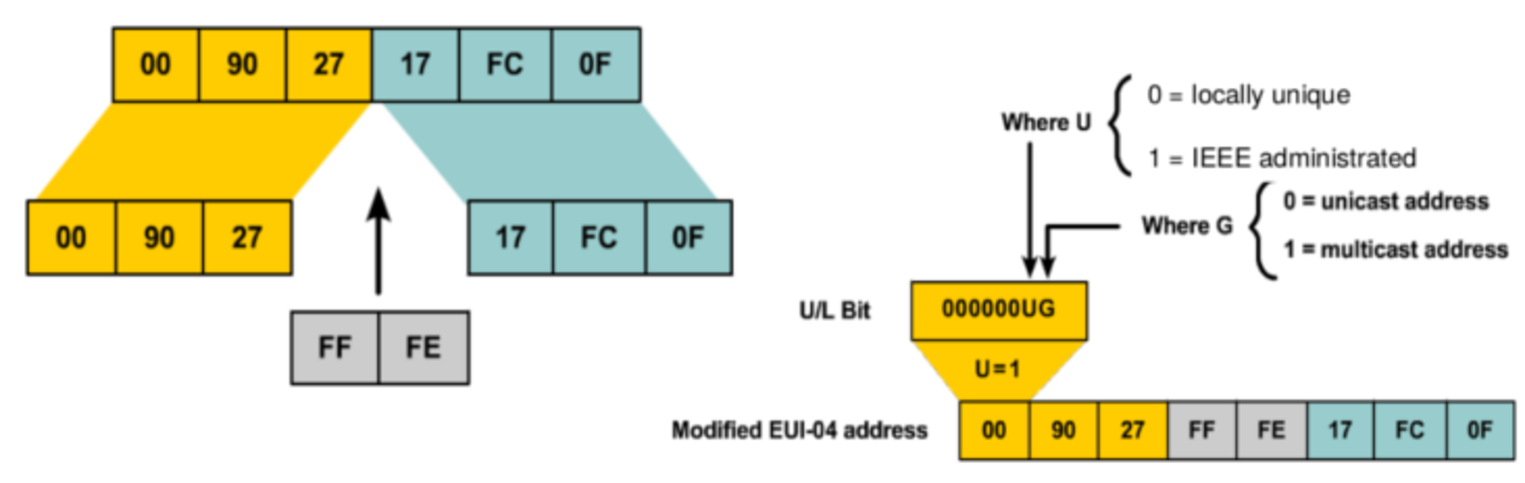
\includegraphics[width=0.7\linewidth]{images/eui-64.pdf}
	\caption{EUI-64 Adresse}
\end{figure}

\begin{figure}[h]
	\centering
	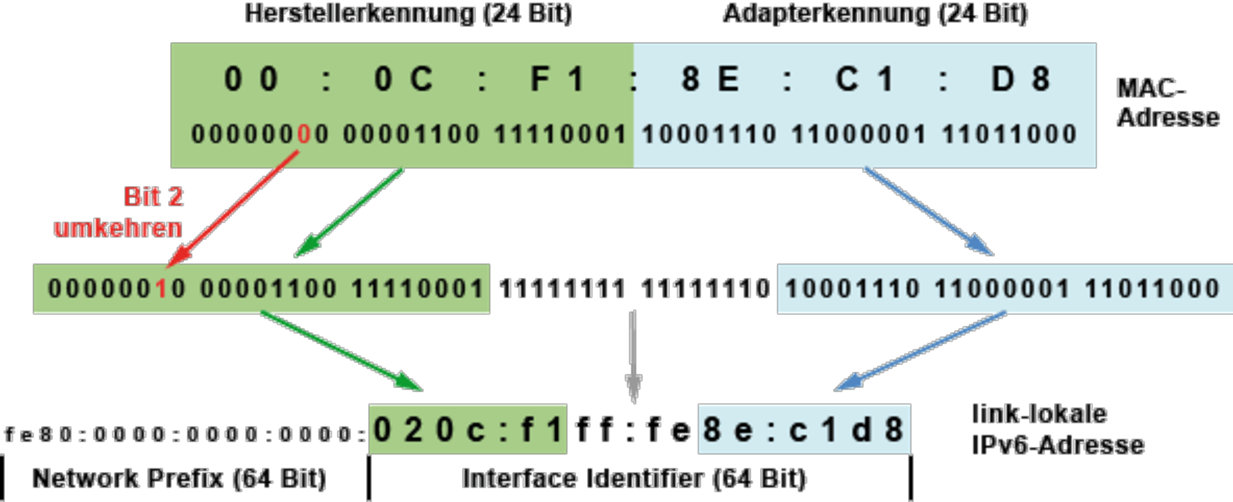
\includegraphics[width=0.7\linewidth]{images/mac_ipv6.pdf}
	\caption{Adressumsetzung von EUI-64 in IPv6 Adresse}
\end{figure}

\paragraph{Privacy Extension}
Privacy Extensions ist eine Erweiterung SLAAC von IPv6, um IPv6-Adressen zu bilden, die keinen Rückschluss auf die Client MAC Adresse zulassen. Inzwischen gehört die Privacy Extension zum Default in fast allen Betriebssystemen. Die nötigen 64 Bit werden bei der Privacy Extension zufällig generiert. (kein FF:FE) Zum aktuellen NTP-Zeitstempel mit 64 Bit kommt die MAC-Adresse hinzu und dann macht man daraus einen SHA1-Hash mit einer Länge von 64 Bit. Fertig ist der "zufällige" Interface Identifier.


\subsection{DHCPv6}
Der Client sendet ein DHCP Request an die Multicast Adresse FF05::1:3
\subsubsection{Stateless}
Der Client konfiguriert sich eine IPv6 Adresse selbständig und bezieht nur Zusatzoptionen wie z.B der DNS Server vom DHCP.

\subsubsection{Stateful}
DHCPv6 im stateful Mode ist weitgehend vergleichbar mit der IPv4 Variante, mit dem Unterschied, dass keine Broadcast Adressen existieren, sondern die Multicastadresse FF02::1:2 dafür verwendet wird.	

\subsection{IPv6 Multicast}
\begin{itemize}
	\item FF00::/8 sind Multicast Adressen (1111 1111)
	\item Die L2 (MAC) Multicast Adresse wird wie folgt gebildet: 33:33:<letzte 32 Bit der IPv6 Multicast Adresse>
\end{itemize}

\begin{tabu} to \linewidth {|l|l|l|}
	\hline
	Adress 	& Scope & Meaning \\ 
	\hline\hline
	FF01::1		& Node Local	& All Nodes  \\ 
	\hline
	FF02::1		& Link Local	& All Nodes \\ 
	\hline
	FF01::2		& Node Local	& All Routers \\ 
	\hline
	FF02::2		& Link Local	& All Routers \\ 
	\hline
	FF05::2		& Site Local 	& All Routers  \\ 
	\hline
	FF02::1:FFXX:XXXX	& Link Local 	& Solicited Node  \\ 
	\hline
\end{tabu}

\begin{figure}[h]
	\centering
	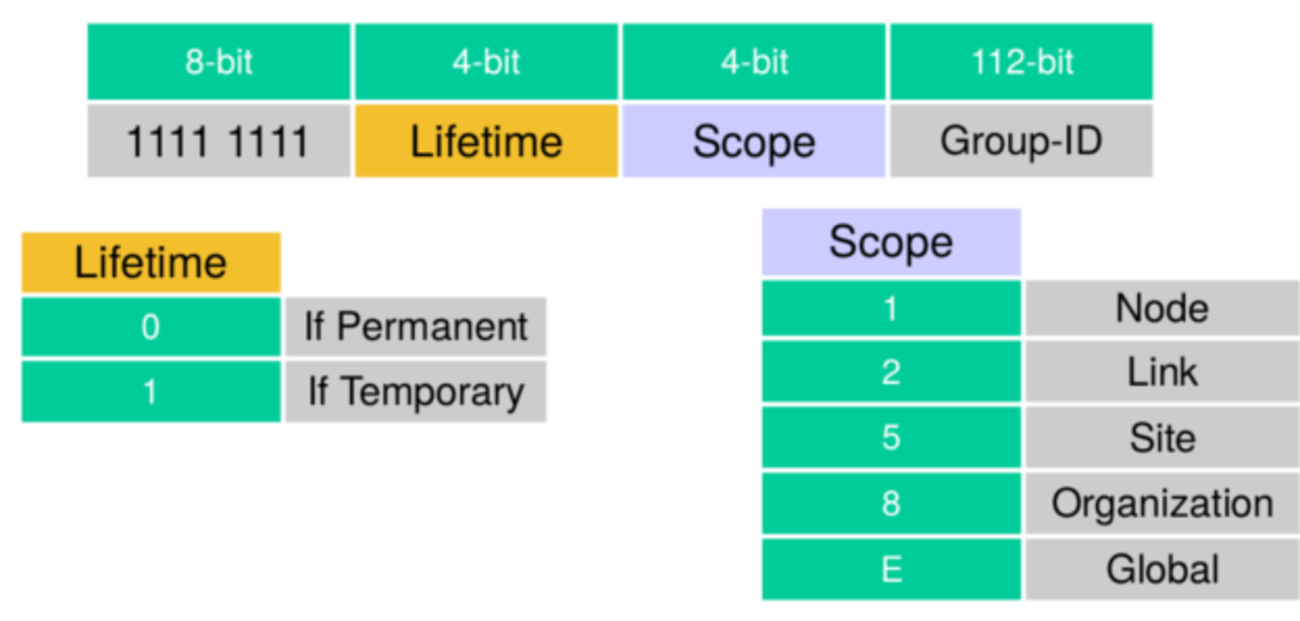
\includegraphics[width=0.4\linewidth]{images/ipv6_multicast.pdf}
	\caption{Adressumsetzung von EUI-64 in IPv6 Adresse}
\end{figure}

\subsubsection{Solicited Node Multicast Address berechnen}
Jede IPv6 Unicast und Anycast Adresse besitzt eine Solicited Node Multicast Adresse. (Diese sind unter "Joined group addresses" zu finden)
\begin{enumerate}
	\item In der Mitte der MAC-Adresse FF:FE einschieben. Die 48Bit lange MAC Adresse wird somit in zwei 24Bit lange Teile unterteilt und um 16Bit erweitert. Das Resultat ist der EUI64
	\item Der Adresse ff02:0000:0000:0000:0000:0001:ffxx:xxxx die letzten 24Bit rsp. 6 Hex Zeichen des EUI64 ersetzen.
\end{enumerate}
\begin{figure}[h!]
	\centering
	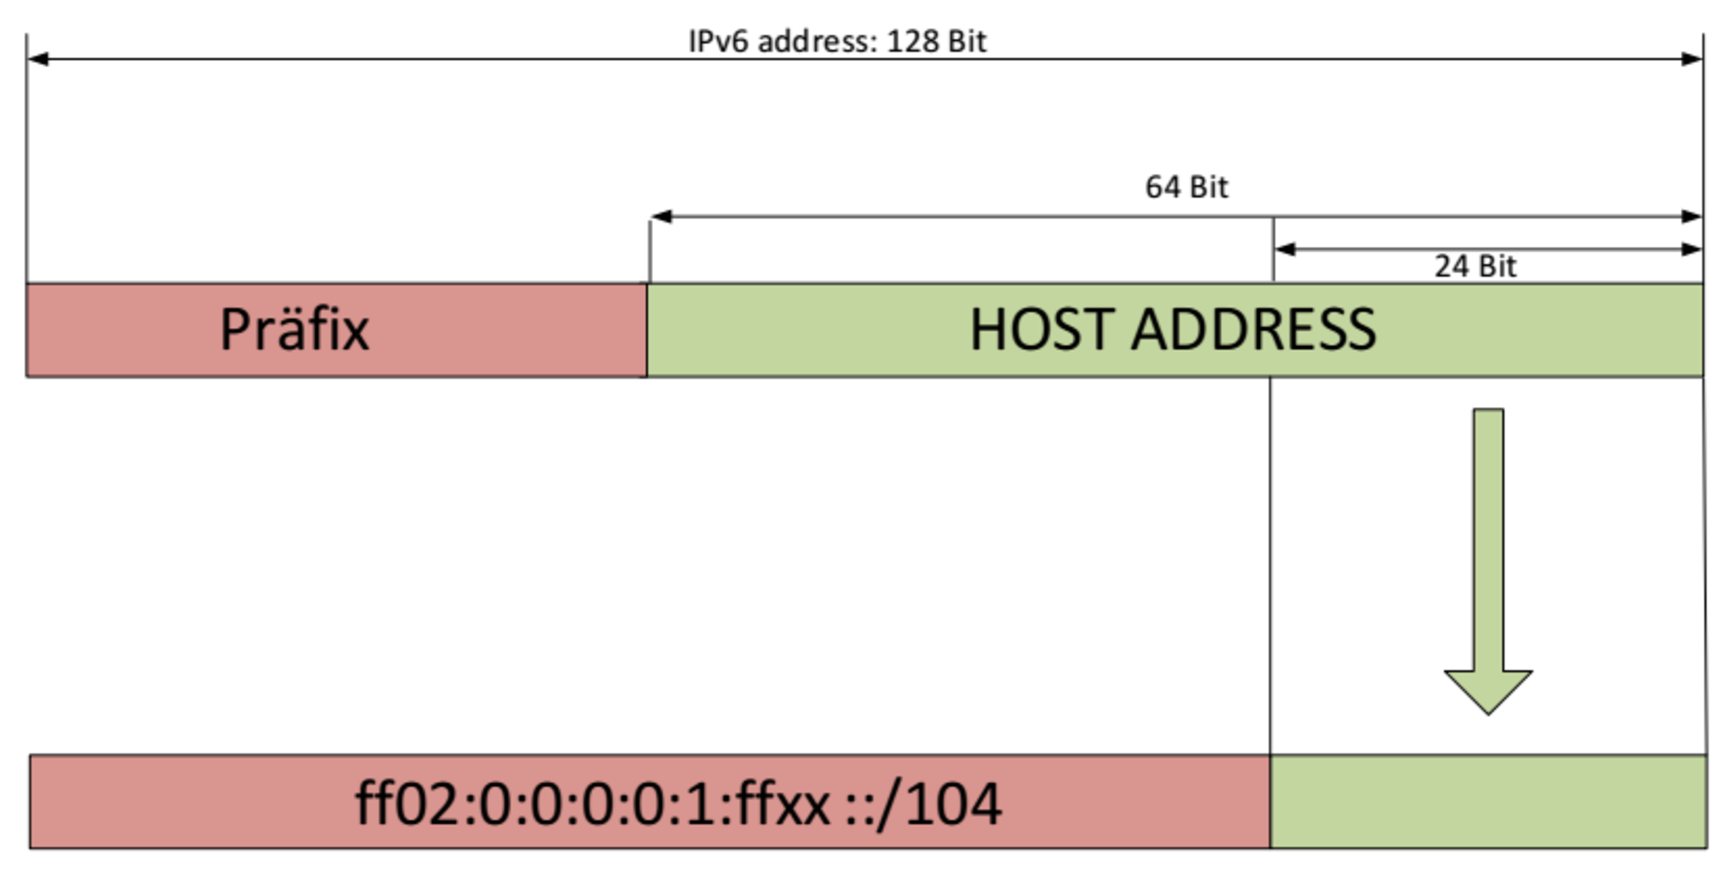
\includegraphics[width=0.4\linewidth]{images/solicited_node_multicast.pdf}
	\caption{Solicited Node Multicast Adress}
\end{figure}

\subsection{Netzwerk Adress Schemas}
\begin{description}
	\item[ULA: Unique Link Local only (nicht empfohlen)] \hfill \\
	Dieses Schema ist kann man mit dem IPv4 Ansatz vergleichen. Die Adressen sind nur lokal signifikant und werden ins Internet ge-NAT-ed. Dieser Ansatz hat ebenfalls den Nachteil, dass es aktuell keine guten IPv6 NAT Lösungen gibt.
	\item[ULA \& Global (nicht empfohlen)] \hfill \\
	Jeder Client hat eine ULA und globale Adresse. Mittels SAS (Source Address Selection) wird bestimmt, welche Adresse für die Kommunikation verwendet wird. 
	\item[Global (empfohlen)] \hfill \\
	Alle Clients haben nur eine global ansprechbare Adresse. Einziger Nachteil ist, dass man somit die Netzwerk Topologie nach aussen nicht versteckt.
\end{description}

\subsection{Adresszuordnung}
\begin{description}
	\item[Stateless Autoconfiguration] Adresszuordnung via SLAAC.
	\item[Stateless Autoconfiguration + stateless DHCP] DHCP wird verwendet um DNS Informationen zu verteilen
	\item[Stateful Autoconfiguration] Ähnlich wie DHCP bei IPv4 (Client sendet DHCP Solicit Message an die All-DHCP-Agents Multicast Adresse)
	\item[Statische Adresszuordnung] Alles manuell
\end{description}

\subsection{ICMPv6: Internet Controll Message Protocol V6}
ICMPv6 wird verwendet, um folgende Nachrichten zu versenden.

\begin{description}
	\item[NDP: Neighbor Discovery Protocol] Ersatz für ARP (Address Resolution Protocol) unter IPv4 und wird dazu benutzt um IPv6 Adressen in Hardwareadressen (L2) aufzulösen.
	\item[RARP: Reverse Address Resolution Protocol] Ermöglicht die Zuordnung von Hardwareadressen zu Internetadressen
	\item[IGMP: Internet Group Management Protocol] Dient der Organisation von Multicast Gruppen. IGMP existiert nur unter IPv4.
	\item[MLD: Multicast Listener Discovery] Ist das IPv6 Pendant zu IGMP. Es wird also genutzt um Multicast Abonnements zu verwalten.
\end{description}

\subsection{Neighbor Discovery / Router Discovery}
Mit Neighbor Discovery wird herausgefunden, ob eine IPv6 Adresse unique ist. Mit Router Discovery wird das Default Gateway für eine eine Station evaluiert.
\begin{enumerate}
	\item ICMP Type Feld 135 = Neighbor Solicitation
	\begin{itemize}
		\item Ein Neighbor Solicitation Nachricht wird gesendet, um die Hardwareadresse (Link Local Address) eines Nachbars ausfindig zu machen. Die Zieladresse ist dabei die IPv6 Multicast Adresse. (nicht wie bei ARP an die Broadcast Adresse)
	\end{itemize}
	\item ICMP Type Feld 136 = Neighbor Solicitation Advertisement. Ist die Antwort auf auf die Neighbor Solicitation und beinhaltet die Link Local Addresse (MAC Pendant) der Station.
	\begin{itemize}
		\item Die Meldungen werden auch verwendet um herauszufinden ob eine IPv6 Adress unique ist.
	\end{itemize}
	\item ICMP Type Feld 133 = Router Solicitation 
	\begin{itemize}
		\item Hiermit bittet eine Station um ein Router Advertisement
		\item Ein Client sendet eine RS an die All-Routers Multicast Adresse
		\item Werden von einer Station beim Aufstarten versendet, damit nicht auf das nächste Update Intervall gewartet werden muss
	\end{itemize}
	\item ICMP Type Feld 134 = Router Advertisement
	\begin{itemize}
		\item Hiermit machen sich Router im Netz bekannt und verbreiten Informationen für die IP-Autokonfiguration (SLAAC).
		\item Werden periodisch oder auf Anfrage (Router Advertisement) von einem IPv6 konfigurierten Router Interface an eine Multicast Adresse versendet. (All Node Multicast der Clients) 
		\item Beinhaltet Hop Limit, Router Lifetime (Default Router für max $2^{16}s \approx 18h$), Erreichbarkeits Timeout Preferierter, Auflösuns-Timeout Router (pref), Proxy (ja, nein) 
		\item Auf diese Weise erfahren alle Hosts die Adresse des Default-Routers und die link-lokalen und globalen Präfixe.
	\end{itemize}
	\item Neighbor Cache:  Der Neighbor-Cache entspricht dem ARP-Cache unter IPv4.
\end{enumerate}

\subsection{Ablauf}
\begin{enumerate}
	\item Router 1 (2001:db8::1/64) will Router 2(2001:db8::2/64) eine Meldung senden
	\item Router 1 berechet die Solicited Node Multicast Adresse von Router 2 (ff02::1:FF00:0002)
	\item Router 1 sendet eine Neighbor Solicitation (135) an die berechnete Solicited Node Multicast. Er bittet damit Router 2 um dessen Link Layer Adresse
	\item Der Router 2 antwortet mit seiner Link Layer Adresse mit einem Neighbor Advertisement (136)
\end{enumerate}


\subsection{DAD: Optimistic Duplicate Address Detection}
DAD ist eine Erweiterung von Neighbor Discovery und SLAAC mit dem Ziel dass eine IPv6 Adresse unique ist. Ein Client mit der Source Adresse ::/0 (noch nicht konfiguriert) sendet an \textbf{seine} Solicited Node Multicast Adresse eine Neighbor Solicitation und fragt ob die Adresse, die er sich zuweisen möchte, schon besetzt ist.

\section{Optische Netzwerke / Fiber}
Es gibt 6 verschiedene Bänder (Kabelstandards) mit unterschiedlichen Wellenlängen die sich in der Dämpfung und somit in der Reichweite unterscheiden. Je höher die Dämpfung, desto kleiner ist folglich die Reichweite. Ein optisches Kabel darf nicht zu viel gebogen werden, da ansonsten der Winkel der Lichtwelle so spitz wird, dass das Signal in den Mantel durchgeht. Der Winkel, wie eine Lichtwelle auf den Mantel aufprallt, muss so gewählt sein, dass die Welle vom Mantel reflektiert wird. In ein optisches Kabel darf niemals hinein geschaut werden.

\begin{figure}[h]
\centering
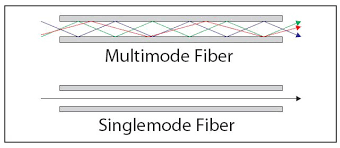
\includegraphics[width=0.4\linewidth]{images/singlemode_multimode}
\caption{Singlemode und Multimode Fasern}
\end{figure}

\begin{description}
	%TODO OEO: Opto Elector Opto 
	\item[Brechungsindex] \hfill \\
	Der Unterschied zwischen dem Brechungsindex vom Glas und dem Mantel sollte möglichst gross sein. Dies unterstützt eine Totalreflexion welche für die verlustfreie Übertragung der Daten nötig ist.
	\item[Multimode Fiber] \hfill \\
	Multimode Fiber erlauben mehr als 500MHz/km und setzen auf mehrere Lichtwellen. In der Schweiz sind zwei Multimode Typen im Umlauf. Der erste Wert ist dabei der Kerndurchmesser und der zweite der Manteldurchmesser.
	\begin{itemize}
		\item 50/125$\mu m$ (grössere Distanz aber teurer)
		\item 62.5/125$\mu m$ (wegen grösserer Kernbreite legen die Lichtstrahlen einen grösseren Weg zurück und sind somit grösserer Dispersion ausgesetzt. )
	\end{itemize}
	\item[Singlemode Fiber] \hfill \\
	Singlemode Fiber erlauben mehr als 100THz-km und haben nur eine einzige Lichtwelle die durch einen 9$\mu m$ dicken Kern geschickt wird.
	\item[Augendiagramm] \hfill \\
	Je grösser der Abstand in der Vertikalen, desto einfacher kann man zwischen 0 und 1 unterscheiden. Je grösser der Abstand in der Horizontalen, desto mehr Zeit hat man das Signal zu samplen. Die horizontale Verschiebung wird Jitter genannt.
	\item[Spleissen] Der Prozess des Zusammenführens zweier Glasfasern wird Spleissen genannt.
	\item[Dispersion] \hfill \\
	Dispersion hat zur Folge, dass ein Signal unscharf wird. (Verbreiterung des Pulses) Je grössere die gewünschte Bandbreite, desto schneller setzt die Dispersion ein. Bei kleineren Bandbreiten können daher grössere Distanzen überwunden werden.
	\begin{itemize}
		\item 2.5Gb/s = 980km
		\item 10Gb/s = 60km
		\item 40Gb/s = 4km
	\end{itemize}
	\item[Reshaping] Unter Reshaping versteht man das verkleinern der Dispersion. Ein verschmiertes Signal wird somit wieder kleiner.
	\item[Re-Timing] Beim Re-Timing wird die Phasenverschiebung beim Samplen optimiert. Das Sampling ist im besten Fall genau in der Mitte des Signals
	\item[PON: Passive Optical Network Architektur] \hfill \\
	Es gibt eine Faser für mehrere Endkunden, welche dann bei einem Verteiler pro Endkunde aufgeteilt wird. Dabei kann man Fasern sparen, alle Endkunden sind aber von der Verfügbarkeit des Verteilers abhängig.
	\item[Point to Point Architektur] \hfill \\
	Hierbei gibt es eine direkte Verbindung zwischen Provider und Endkunde. 
	\item[WDM: Wave Division Multiplexing] \hfill \\
	Mehrere Farben auf eine einzige Glasfaser.
	\item[DWDM: Dense Wave Division Multiplex] \hfill \\
	Dense Wave Division	Multiplexing Systeme legen sehr viel mehr Wellenlängen auf ein kleineres Spektrum, was die Gesamtkapazität	stark erhöht. Die	Kosten von DWDM	Systemen	sind denn auch deutlich	höher.	
	\item[CWDM: Coarse Wave Division Multiplex] \hfill \\
	Coarse Wave Division Multiplexing Systeme haben einen grösseren Kanalabstand und können deshalb mit günstigerer Elektronik hergestellt werden. CWDM Systeme überbrücken deutlich kleinere Distanzen als DWDM und 
	werden deshalb von allem im Städte (Metro) Bereich eingesetzt. Ebenso sind die Geschwindigkeiten auf 2.5 Gbps 
	beschränkt.
\end{description}

\begin{figure}[h]
	\centering
	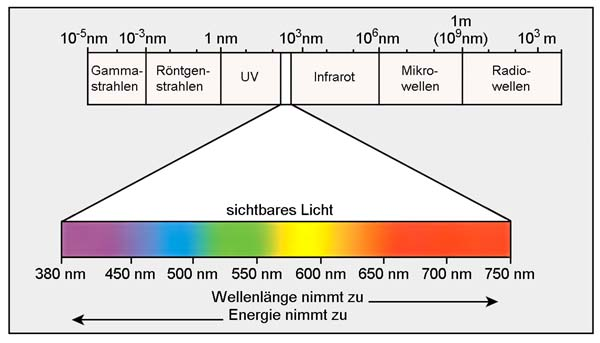
\includegraphics[width=0.4\linewidth]{images/wellenlaengen.jpg}
	\caption{Singlemode und Multimode Fasern}
\end{figure}

\[ C = \lambda \cdot v \]
\begin{itemize}[label=]
	\item $C$ = Lichtgeschwindigkeit
	\item $\lambda$ = Wellenlänge (nm)
	\item $v$ = Frequenz 
\end{itemize}

\subsection{Power Budget}
Das optische Budget wird in dB gemessen und kann wie folgt berechnet werden. Aus dem optischen Budget kann anschliessend die maximale Kabellänge berechnet werden, indem man das optische Budget durch die Dämpfung (db/km) teilt.
\[
	\text{Optical Power Budget (dB)} = \text{Power of Sender(dB)} - {Sensitivity of Receiver(dB)}
\]
\begin{itemize}[label=]
	\item SR: Short Reach = 6dB
	\item IR: Intermediate Reach = 13dB
	\item LR: Long Reach = 26dB
\end{itemize}

\section{Storage Network}
\begin{description}
	\item[DAS: Direct Attached Storage] Direkt angehängtes Storage an einem Server. Kann nur von diesem einen Server angesprochen werden.
	\item[NAS: Network Attached Storage] Ist ein konfigurierbarer Datenspeicher um in einem Netzwerk Speicherplatz zur Verfügung zu stellen. Dabei ist an NAS an keinen Server gebunden, sondern als eigenständige Einheit zu sehen.
	\item[SAN: Storage Area Network]  \hfill \\ Ist ein Datenspeicher Netzwerk in dem grosse Datenmengen gespeichert werden. Das Storage wird vom Server getrennt. Server übertragen die Daten via iSCSI auf Block Level in das SAN. 
	\item[SCSI: Small Computer System Interface] SCSI ist ein Protokoll zur Steuerung der Kommunikation zwischen Massenspeicher und Controller. 
	\item[iSCSI: Internet SCSI] iSCSI ist ein L5 Protokoll, das die Übertragung von SCSI-Befehlen über ein TCP/IP-Netzwerk regelt
	\item[LUN: Logical Unit Number] Für die eindeutige Identifizierung eines einzelnen SCSI-Gerätes wird die LUN verwendet, welche 64 Bit lang ist
	\item[RAID: Reduntant Array of Idependent Disks] \hfill
	\begin{itemize}
		\item RAID 0: Keine ausfallsicherheit, dafür schnelle Lese und Schreibgeschwindigkeit
		\item RAID 1: Ausfallsicher, aber teuer, da immer nur die hälfte der verfügbaren Kapazität verwendet werden kann
		\item RAID 5: Ausfallsicher, je nach Controller aber langsame Schreibgeschwindigkeit. RAID 5 ist eine gute Kombination aus Datensicherheit und Speicherausnutzung (min 3 Platten nötig, wobei nur eine Platte ausfallen darf)
		\item RAID 6: Sehr ausfallsicher (mindestens 4 Platten nötig, wobei 2 davon ausfallen dürfen)
		\item RAID 0+1: RAID 0 wird mit RAID 1 gespiegelt
		\item RAID 1+0: RAID 1 wird mit zweitem RAID 1 via RAID 0 verbunden
	\end{itemize}
\end{description}

\begin{figure}[h]
	\centering
	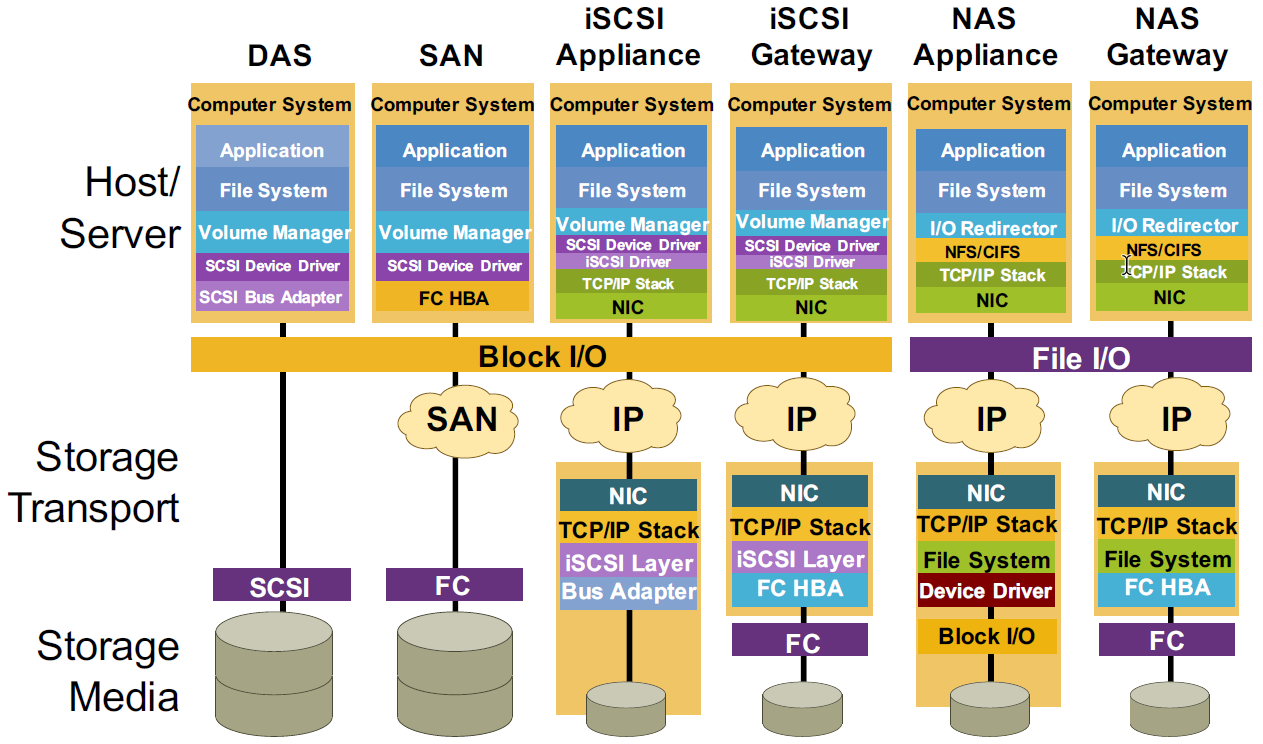
\includegraphics[width=0.7\linewidth]{images/storage_overview}
	\caption{Fibre Channel Port Übersicht}
\end{figure}

\subsection{FC: Fibre Channel}
FC überträgt SCSI Befehle und Daten in serieller Form in ein SAN. Bei Fibre Channel wird davon ausgegangen, dass es kein Paketverlust gibt

\subsubsection{Ports}
\begin{itemize}
	\item N Port (Node): Gerät ist direkt an eine Switched Fabric angeschlossen oder P2P mit einem anderen Gerät
	\item F Ports (Fabric): F Ports sind immer auf einer Switched Fabric. Ist mit einem N Port verbunden
	\item E Ports (Expansion): Verbindung zu einem anderen SAN Switch
	\item L Ports (Loop)
\end{itemize}

\begin{figure}[h]
	\centering
	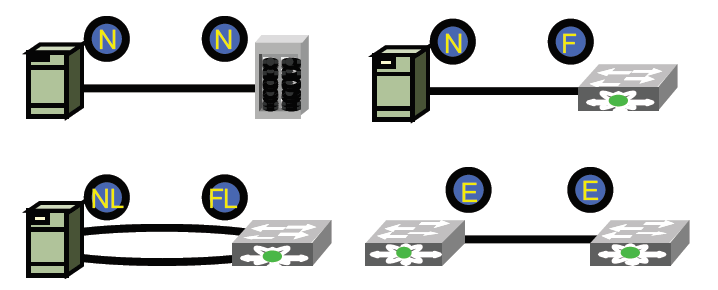
\includegraphics[width=0.5\linewidth]{images/fc_ports}
	\caption{Fibre Channel Port Übersicht}
\end{figure}

\subsubsection{Komponenten}
\begin{itemize}
	\item Fabric: Objekt, welches N Port verbindet. Kann entweder Point-to-Point, Arbitrated Loop (bis zu 127 Ports in einem Ring verbunden) oder Switches (bis zu $2^{24}$ Switches miteinander verbunden) sein
	\item Fabric Controller (Adresse FF FF FD): Jeder Switch hat einen Fabric Controller. Verantwortlich fü das Verhalten des Fabrics, das Routing und das Setup von Class 1 Verbindungen
	\item Directory Server / Name Server (Adresse FF FF FC) Ist eine zentrale Registrierungsstelle für alle Fibre-Channel Komponenten innerhalb eines Netzwerks. Ein N-Port hat die Möglichkeit die Informationen aus einem Directory abzufragen.
\end{itemize}

\begin{figure}[h]
	\centering
	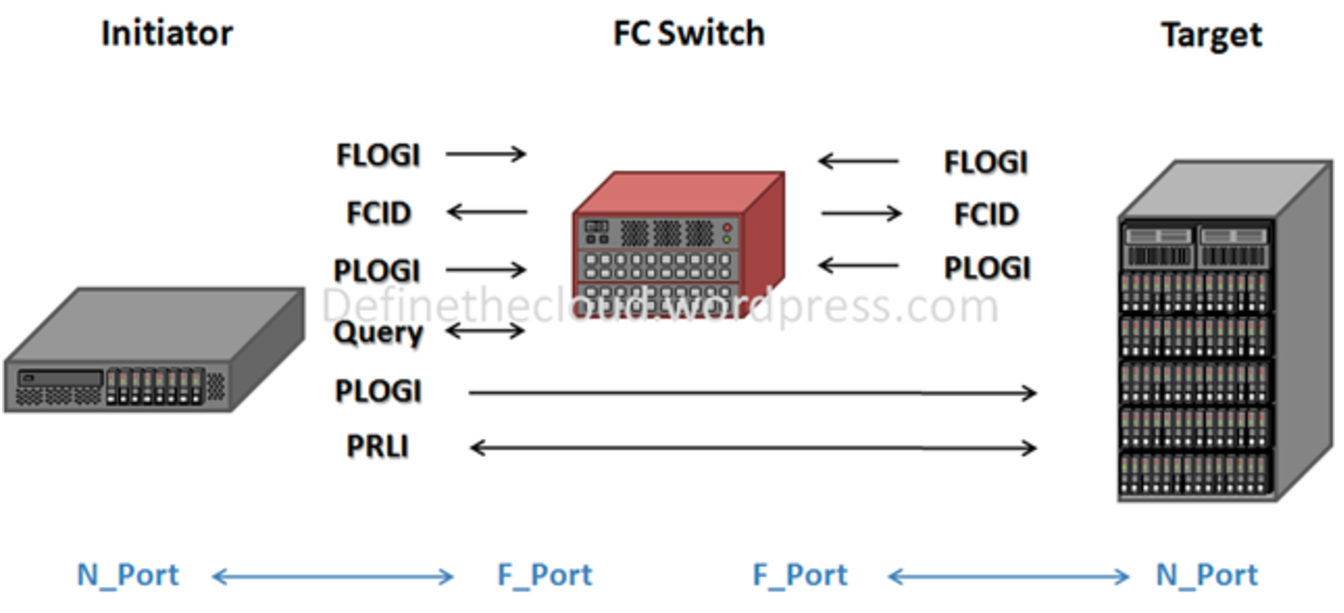
\includegraphics[width=0.7\linewidth]{images/flog_plogi}
	\caption{Fibre Channel Übersicht}
\end{figure}

\begin{description}
	\item[FLOGI: Fabric Login] \hfill \\
	Durch das FLOGI meldet sich ein N-Port bei der zuständigen Fabric an. (auf dem F-Port). Der Initiator oder das Target macht sich im FC Netzwerk bekannt und meldet sich beim Nameserver an, damit er für andere sichtbar und erreichbar wird.
	\item[PLOGI: Port Login] \hfill \\ 
	Das PLOGI ist bevor jeder Kommunikation zwischen zwei N-Ports notwendig. Wird für die Anmeldung eines Initiator beim Target und für die Registrierung am Name Server verwendet. Geht einer Datenübertragung voraus und ist mit einem TCP 3-way Handshake vergleichbar.
\end{description}

\begin{figure}[h]
	\centering
	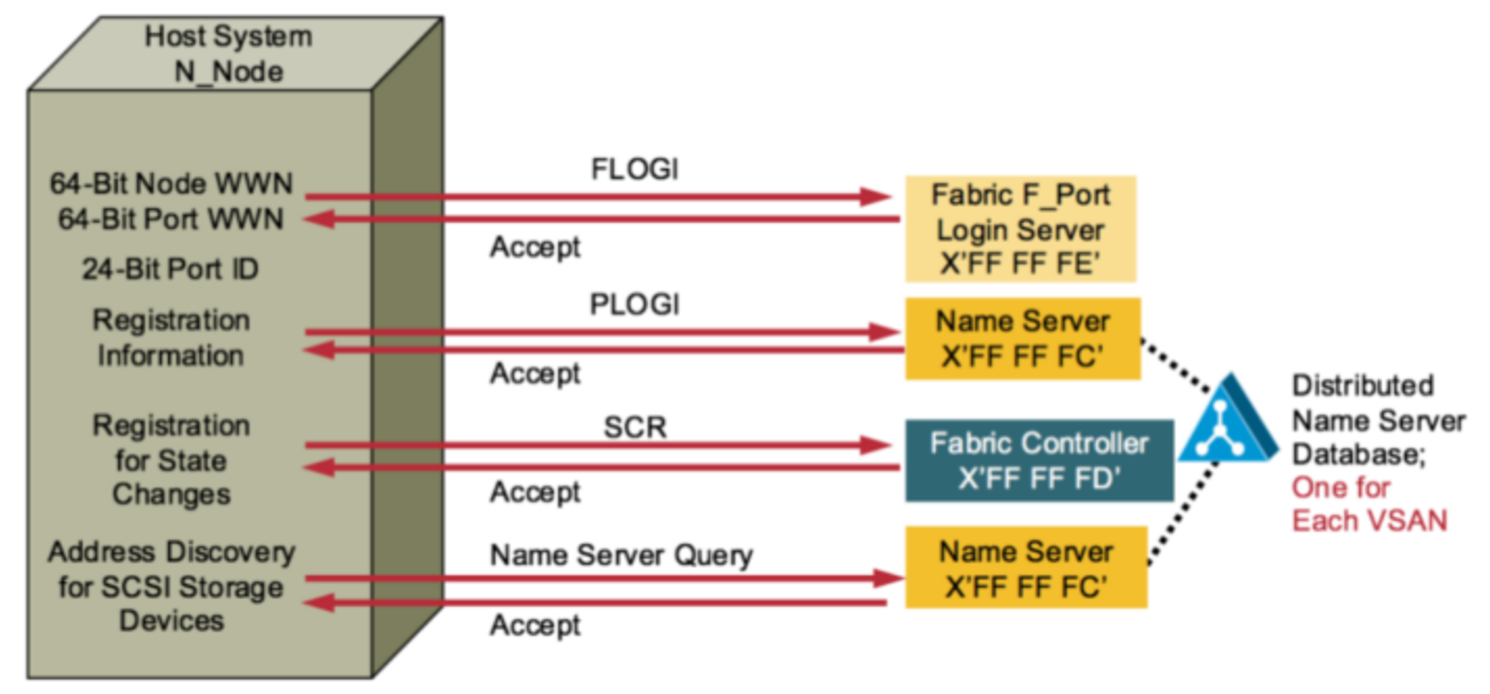
\includegraphics[width=0.7\linewidth]{images/flog_plogi_2}
	\caption{Fibre Channel Übersicht}
\end{figure}


\subsubsection{Layers}
\begin{description}
	\item[L0: Physical Interface] Definiert die physischen Interfaces Eigenschaften (Kabel,	Stecker, Signal	Rate)
	\item[L1: Transmission Code] Definiert wie Eigenschaften Encoded/Decoded übertragen werden
	\item[L2: Signaling Protocol] Definiert wie Informationen übertragen werden (Frames, Sequenzen, Login Sessions)
	\item[L3: Common Services] Platzhalter für zukünftige Funktionen
	\item[L4: ULP] Definiert wie die verschiedenen Protokolle in Fibre Channel gebraucht werden (SCI; IP FICON)
\end{description}

\subsubsection{WWN: World Wide Name}
Der WWN ( World Wide Name) ist eine 64 oder 128Bit lange Kennung zum Identifizieren eines einzelnen Ports. 

\subsection{Buffer Credits}
Pro Netzabschnitt sind eine bestimmte Anzahl Buffer Credits verfügbar. Diese werden beim herausgehen aus dem Interface heruntergezählt und erst beim Ankommen des Tokens zurück zum Ursprungsinterface wieder inkrementiert.

\subsection{FSPF: Fabric Shortest Path First}
FSPF routet den Traffic gemäss der Ziel Domain Id aus der FCID.


\appendix

% Code Listings
\lstlistoflistings

% List of figures
\listoffigures

% List of tables
\listoftables

% Bibliography
\bibliographystyle{plain} 
\bibliography{literatur}

\end{document}